\documentclass[a4paper]{article}
\usepackage[spanish]{babel}
\usepackage[utf8]{inputenc}
\usepackage{charter}   % tipografia
\usepackage{graphicx}
%\usepackage{makeidx}
\usepackage{paralist} %itemize inline
\usepackage{pdfpages}
\usepackage[ruled,vlined]{algorithm2e}
\usepackage{amsmath}

%\usepackage{float}
%\usepackage{amsmath, amsthm, amssymb}
%\usepackage{amsfonts}
%\usepackage{sectsty}
%\usepackage{charter}
%\usepackage{wrapfig}
%\usepackage{listings}
%\lstset{language=C}


\usepackage{color} % para snipets de codigo coloreados
\usepackage{fancybox}  % para el sbox de los snipets de codigo

\definecolor{litegrey}{gray}{0.94}

% \newenvironment{sidebar}{%
% 	\begin{Sbox}\begin{minipage}{.85\textwidth}}%
% 	{\end{minipage}\end{Sbox}%
% 		\begin{center}\setlength{\fboxsep}{6pt}%
% 		\shadowbox{\TheSbox}\end{center}}
% \newenvironment{warning}{%
% 	\begin{Sbox}\begin{minipage}{.85\textwidth}\sffamily\lite\small\RaggedRight}%
% 	{\end{minipage}\end{Sbox}%
% 		\begin{center}\setlength{\fboxsep}{6pt}%
% 		\colorbox{litegrey}{\TheSbox}\end{center}}

\newenvironment{codesnippet}{%
	\begin{Sbox}\begin{minipage}{\textwidth}\sffamily\small}%
	{\end{minipage}\end{Sbox}%
		\begin{center}%
		\vspace{-0.4cm}\colorbox{litegrey}{\TheSbox}\end{center}\vspace{0.3cm}}



\usepackage{fancyhdr}
\pagestyle{fancy}

%\renewcommand{\chaptermark}[1]{\markboth{#1}{}}
\renewcommand{\sectionmark}[1]{\markright{\thesection\ - #1}}

\fancyhf{}

\fancyhead[LO]{Sección \rightmark} % \thesection\ 
\fancyfoot[LO]{\small{Aldasoro Agustina, Bouz\'on Mar\'ia Bel\'en, Cairo Gustavo Juan}}
\fancyfoot[RO]{\thepage}
\renewcommand{\headrulewidth}{0.5pt}
\renewcommand{\footrulewidth}{0.5pt}
\setlength{\hoffset}{-0.8in}
\setlength{\textwidth}{16cm}
%\setlength{\hoffset}{-1.1cm}
%\setlength{\textwidth}{16cm}
\setlength{\headsep}{0.5cm}
\setlength{\textheight}{25cm}
\setlength{\voffset}{-0.7in}
\setlength{\headwidth}{\textwidth}
\setlength{\headheight}{13.1pt}

\renewcommand{\baselinestretch}{1.1}  % line spacing


% \setcounter{secnumdepth}{2}
\usepackage{underscore}
\usepackage{caratula}
\usepackage{url}




\begin{document}


\thispagestyle{empty}
\materia{M\'etodos Num\'ericos}
\submateria{Segundo Cuatrimestre de 2014}
\titulo{Trabajo Práctico III}
\subtitulo{Develando la mentira de los megap\'ixeles}
\integrante{Aldasoro Agustina}{86/13}{agusaldasoro@gmail.com}
\integrante{Bouz\'on Mar\'ia Bel\'en}{128/13}{belenbouzon@hotmail.com}
\integrante{Cairo Gustavo Juan}{89/13}{gjcairo@gmail.com}

\maketitle
\newpage

\thispagestyle{empty}
\vfill
\begin{abstract}
En el presente trabajo se pretende analizar y comparar distintas alternativas que pretenden dar respuesta al problema de demosaicing. Para ello, las mismas serán implementadas y sometidas a experimentación sobre fotografías crudas sintéticas específicamente seleccionadas para poner de manifiesto las ventajas e inconvenientes del empleo de cada método. \\
\end{abstract}

\textbf{Palabras clave:} \\
$\bullet$ Filtro Bayer \\
$\bullet$ Demosaicing \\
$\bullet$ Interpolaci\'on \\
$\bullet$ Artifacts \\



\thispagestyle{empty}
\vspace{3cm}
\tableofcontents
\newpage


%\normalsize
\newpage

\section{Introducci\'on Te\'orica}

Promediando la década de 1990 comenzaron a introducirse al mercado las cámaras digitales de uso hogareño, empezando a sustituir desde entonces a las ampliamente difundidas cámaras de film. 
Mientras que estas últimas capturaban la imagen de forma mecánica y sin intercesión de un procesamiento digital, las cámaras electrónicas emplearon una nueva tecnología. Esta tecnolog\'ia distingue entre en el momento de obtención de un conjunto de datos cerca del objetivo – donde se obtiene una imagen que llamaremos “\textit{cruda}” – y una etapa de procesamiento automático conjunto a la reconstrucción de la imagen final. \\

En el presente trabajo nos interesará analizar un fragmento de dicha etapa conocido como \emph{demosaicing}. Para entender de qué consta, es menester comprender previamente la forma en que se capturan las imágenes al utilizar cámaras digitales.

Este tipo de cámaras poseen un sensor CCD compuesto de una matriz de elementos fotosensibles, cada uno de los cuales es capaz de captar la intensidad de la luz que llega a ese punto a través de la lente. 

La tarea de capturar todos los colores reflejados por el objetivo que se quiere fotografiar no está encomendada a ninguna posición en particular, sino que cada una de ellas tiene asignada – de acuerdo a algún patrón definido  – la captura de la información perteneciente a un solo color. Cada p\'ixel de la imagen va a estar dividido en tres canales ya que la vamos a almacenar, en nuestro caso de estudio, mediante RGB (Red, Green, Blue).

El patr\'on que determina qué color será capturado por cada fotosensor es denominado \emph{Color Filter Array} y var\'ia de acuerdo al fabricante de c\'amaras. Existen diversos patrones, en nuestro trabajo nos centraremos en el \textbf{Filtro Bayer}, ya que es un filtro com\'unmente usado debido a que la cantidad de informaci\'on que brinda sobre el canal verde - al cual el ojo humano es más sensible por encontrarse en el centro de su espectro visual y es el canal que brinda mayor informaci\'on sobre la luminiscencia -  duplica a cada uno de los otros dos.

\textcolor{red}{*insertar imágenes por aquí y por allá* (?
}

\begin{figure}[h!]
	\caption{Bayer CFA}
	\begin{center}
	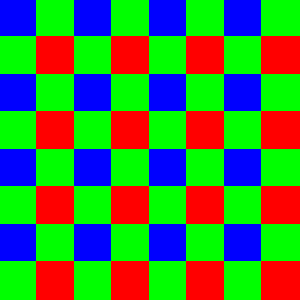
\includegraphics[scale=0.36]{imagenes/BayerFilter}
	\label{Bayer}
  \end{center}
\end{figure}


Ahora bien, esto genera una imagen que se aproxima a la realidad sólo en parte ya que para cada p\'ixel de la imagen tenemos la informaci\'on de s\'olo uno de sus tres canales. A causa de esto es que la misma debe ser reconstruida algorítmicamente, interpolando los valores de los colores que no fueron almacenados explícitamente para cada pixel.


En este punto adquieren relevancia las diferentes propuestas de reconstrucción de la imagen original. Esto conlleva la ejecución de diversos procedimientos, entre los que se encuentran el demosaicing, el análisis del balance de blancos, la curva tonal, la saturación y el contraste y la compresión final de la imagen. Como nuestra propuesta se aboca al primer paso mencionado, exploraremos en el presente trabajo sólo un subconjunto de una serie de variaciones no finita que admiten métodos de debayering como ser la interpolación por asignación de valores próximos, la interpolación bilineal y interpolación direccional.\\

A efectos de nuestro caso de estudio, la imagen bajo el Color Filter Array Bayer la vamos a generar sint\'eticamente, es decir mediante un algoritmo que tome una imagen original y devuelva una imagen de este formato. Esto nos permitir\'a hacer comparaciones entre los m\'etodos y la imagen original, teniendo as\'i un punto de referencia en cuanto a la correctitud de la imagen.

\newpage
\subsection{Inconvenientes de aproximar mediante el Polinomio de Lagrange}


Es nuestra intención exponer ahora el motivo que consideramos suficiente para decidir interpolar los valores ausentes a través de Splines en lugar de hacer uso del polinomio de Lagrange.\\
Sea dada la siguiente muestra: \\
\smallskip


\begin{tabular}{ | c || c | c | c | c | c |c | c | c | c | c | c | c | c | c | c |}
 \hline                 
   x & 1 & 2 & 3 & 4 & 5 & 6 & 7 & 8 & 9 & 10 & 11 & 12 & 13 & 14 \\
 \hline    
y & 10 & 10 & 10& 10& 10& 10& 10& 10& 10& 10& 10& 10& 10& 10 \\
 \hline  
 \end{tabular}

\smallskip

\begin{tabular}{  | c || c | c | c | c | c |c | c | c | c | c | c | c | c | c | c |}
 \hline                 
   x&15& 16 & 17 & 18 & 19 & 20 & 21 & 22 & 23 & 24 & 25 & 26 & 27 & 28\\
 \hline    
y & 10 & 10 & 10& 10& 10& 10& 10& 10& 10& 10& 10& 10& 10& 10 \\
 \hline  
 \end{tabular}
\bigskip
\\
El polinomio de Lagrange que interpola cada uno de esos valores tiene una expresión equivalente al Spline que lo hace, siendo su gráfico el que se muestra a continuación:
\smallskip

\begin{figure}[h!]
	\caption{}
	\begin{center}
	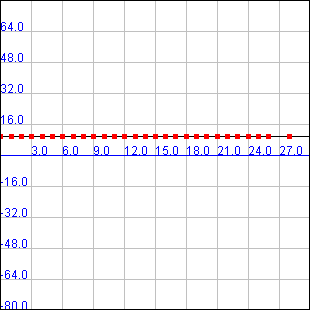
\includegraphics[scale=1]{imagenes/LagrangeSplinesCTE}
	\label{LagrangeSplinesCTE}
  \end{center}
\end{figure}

Supongamos ahora que el resultado de una medición - digamos $x_{12}$ - haya sido calculada con un ruido que represente el 1\% del valor real, modificándose la muestra de la siguiente forma:\\

\smallskip

\begin{tabular}{ | c || c | c | c | c | c |c | c | c | c | c | c | c | c | c | c |}
 \hline                 
   x & 1 & 2 & 3 & 4 & 5 & 6 & 7 & 8 & 9 & 10 & 11 & 12 & 13 & 14 \\
 \hline    
y & 10 & 10& 10& 10& 10& 10& 10& 10& 10& 10& 10& 10,1& 10 & 10\\
 \hline  
 \end{tabular}

 \smallskip

\begin{tabular}{  | c || c | c | c | c | c | c | c | c | c | c | c | c | c | c | }
 \hline                 
   x&15& 16 & 17 & 18 & 19 & 20 & 21 & 22 & 23 & 24 & 25 & 26 & 27 & 28\\
 \hline    
y & 10 & 10 & 10& 10& 10& 10& 10& 10& 10& 10& 10& 10& 10& 10 \\
 \hline  
 \end{tabular}

\bigskip

 En este caso se obtendría el gráfico representado en la Figura \ref{LagrangeX12a101} para el polinomio de Lagrange (escalado en la Figura \ref{LagrangeX12a101(zoomOut)})y el que se ilustra en la Figura \ref{SplinesX12a101} para el obtenido mediante Splines.\\

\begin{figure}[h!]
	\caption{}
	\begin{center}
	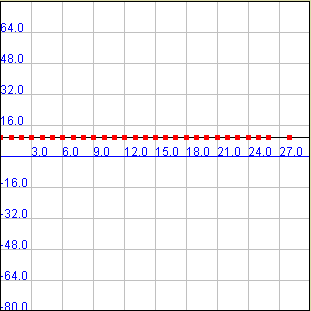
\includegraphics[scale=1]{imagenes/SplinesX12a101}
	\label{SplinesX12a101}
  \end{center}
\end{figure}

\begin{figure}
	\caption{}
	\begin{center}
	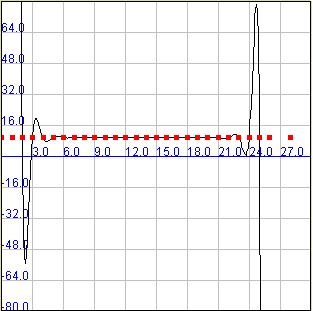
\includegraphics[scale=1]{imagenes/LagrangeX12a101}
	\label{LagrangeX12a101}
  \end{center}
\end{figure}

\begin{figure}
	\caption{}
	\begin{center}
	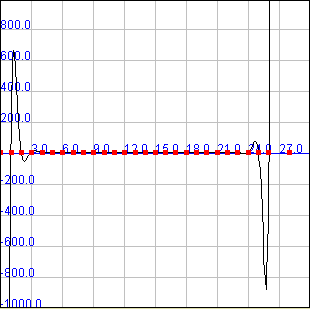
\includegraphics[scale=1]{imagenes/LagrangeX12a101(zoomOut)}
	\label{LagrangeX12a101(zoomOut)}
  \end{center}
\end{figure}

Como se puede observar, para la construcción del Spline el cambio en un valor de la imagen no impactó de una forma apreciable sobre el resto del polinomio. Sin embargo, el nuevo resultado generó un polinomio de Lagrange cuya diferencia con la Figura \ref{SplinesX12a101} es grosera en determinados intervalos.\\ 

Si se profundizara el error de la medición de acuerdo con la tabla presentada a continuación, notaríamos que el polinomio de Lagrange comenzaría a presentar una mayor cantidad de intervalos con valores drásticamente alejados de los dados como referencia. Por otro lado, Splines únicamente presentará variaciones en un entorno de los intervalos cuyos valores hayan sido modificados. Esto se puede  constatar en las Figuras \ref{SplinesX12a20}, \ref{LagrangeX12a20} y  \ref{LagrangeX12a20(zoomOut)}.\\


\begin{tabular}{ | c || c | c | c | c | c |c | c | c | c | c | c | c | c | c | c |}
 \hline                 
   x & 1 & 2 & 3 & 4 & 5 & 6 & 7 & 8 & 9 & 10 & 11 & 12 & 13 & 14 \\
 \hline    
y & 10 & 10& 10& 20& 10& 10& 10& 10& 10& 10& 10& 20& 10 & 10\\
 \hline  
 \end{tabular}

\smallskip

\begin{tabular}{  | c || c | c | c | c | c | c | c | c | c | c | c | c | c | c | }
 \hline                 
   x&15& 16 & 17 & 18 & 19 & 20 & 21 & 22 & 23 & 24 & 25 & 26 & 27 & 28\\
 \hline    
y & 10 & 10 & 10& 10& 10& 10& 10& 10& 10& 10& 10& 10& 10& 10 \\
 \hline  
 \end{tabular}

\begin{figure}
	\caption{}
	\begin{center}
	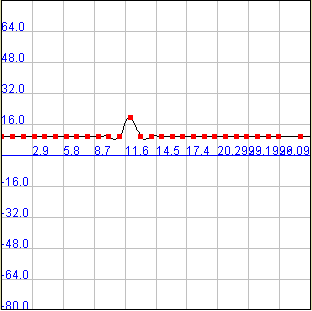
\includegraphics[scale=1]{imagenes/SplinesX12a20}
	\label{SplinesX12a20}
  \end{center}
\end{figure}

\begin{figure}
	\caption{}
	\begin{center}
	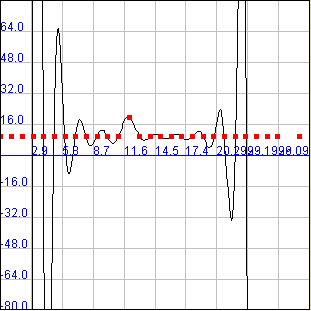
\includegraphics[scale=1]{imagenes/LagrangeX12a20}
	\label{LagrangeX12a20}
  \end{center}
\end{figure}

\begin{figure}
	\caption{$Zoom \ out$ de la Figura \ref{LagrangeX12a20}}
	\begin{center}
	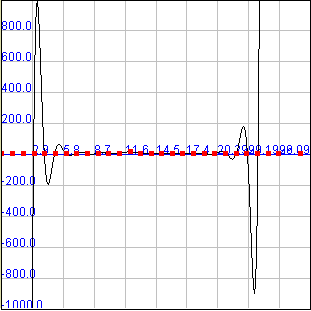
\includegraphics[scale=1]{imagenes/LagrangeX12a20(zoomOut)}
	\label{LagrangeX12a20(zoomOut)}
  \end{center}
\end{figure}

\bigskip

\newpage
En conclusión, el polinomio de Lagrange se comporta de una manera menos predecible estable entre dos variables independientes y no garantiza que en esos intervalos el valor de la función sea cercano a los ya conocidos.\\
La carencia de predictibilidad hace del polinomio de Lagrange una mala alternativa para la interpolación, en comparación con las ventajas proporcionadas por el empleo de Splines.\\




\newpage
\subsection{M\'etricas de comparaci\'on de im\'agenes}

Con el fin de establecer una relaci\'on entre las im\'agenes obtenidas con los distintos m\'etodos y la imagen original es que nace la necesidad de contar con \emph{M\'etricas de comparaci\'on de im\'agenes}.\\

Existen dos m\'etodos dentro de los mecanismos usados:

\emph{Subjetivos:} Son los conceptos que una persona puede detectar visualmente.

\emph{Objetivos:} Son operaciones matem\'aticas en el dominio bidimensional o tridimensional de im\'agenes orientados a determinar la variaci\'on presente en una imagen.\\

Las métricas subjetivas u objetivas se pueden usar con comparación respecto a una referencia o sin considerarla.\\

En nuestro caso de estudio, nos vamos a centrar en la comparaci\'on de la imagen original y la obtenida a trav\'es de los distintos m\'etodos. Por esto mismo, vamos a usar m\'etricas que cuenten con una imagen de referencia.\\

 Dos de las m\'etricas m\'as sencillas son el \emph{\textbf{Error cuadr\'atico Medio}} (mse) y \emph{\textbf{Peak signal-to-noise ratio}} (psnr). Ambas cuentan con la capacidad de an\'alisis p\'ixel por p\'ixel.\\

\[
 \textbf{mse} = \frac{1}{mn} \sum_{i=0}^{m-1} \sum_{j=0}^{n-1} [I(x,y) - K(x,y)]^2
\]
  \indent \indent \indent \textit{Donde I y K son imágenes a comparar de tamaño $mxn$.}



\[
 \textbf{psnr} = 10 \log \frac{(2^n-1)^2}{mse} = 10 \log \frac{255^2}{mse}
\]

Otro tipo de medidas a tener en cuenta son las que utilizan indicadores de la imagen similares a los presentes en la visi\'on humana, como es el caso de \emph{\textbf{Structural similarity}} (ssim) que es una funci\'on que depende de la luminiscencia, el contraste y la similitud estructural.

\[
 \textbf{ssim}(x,y) = \frac{(2\mu_x\mu_y+c_1)(2\sigma_{xy}+c_2)}{(\mu_x^2+\mu_y^2+c_1)(\sigma_x^2+\sigma_y^2+c_2)}
\]

\noindent Donde, 

$\mu_x$ es la esperanza de $x$

$\mu_y$ es la esperanza de $y$

$\sigma_x^2$ es la varianza de $x$

$\sigma_y^2$ es la varianza de $y$

$\sigma_{xy}$ es la covarianza entre $x$ e $y$

$c_1 = (k_1L)^2$ ; $c_2 = (k_2L)^2$ son dos variables que estabilizan la divisi\'on con un denominador chico

$L$ es el rango din\'amico de los valores de los p\'ixeles (com\'unmente es $2^{\#bitsPorPixel}-1$)

$k_1 = 0,01$ y $k_2 = 0,03$ por default\\

Las m\'etricas que vamos a utilizar nosotros como m\'etodo de comparacion de im\'agenes son \emph{psnr} y \emph{ssim}. Los cuales calcularemos con sus instrucciones respectivas en Matlab$\textregistered$.

\newpage
\subsection{Artifacts}
\textcolor{red}{Explicar cada artifact y agregar grid}

Como se explicó anteriormente, dos de los tres canales de cada p\'ixel son interpolados algorítmicamente. Si bien los métodos que pueden proponerse a tal fin no son limitados, un subconjunto de ellos producirá imágenes que diferirán considerablemente de las que quisieron ser capturadas originalmente. 

Para evaluar el peso de estas diferencias  existen mecanismos cuantitativos (como los mencionados en el apartado \emph{M\'etricas de comparaci\'on de im\'agenes}) y otros de tipo cualitativo. Un grupo de estos últimos está constituido por la exploración de \textit{artifacts}.

Los \textit{artifacts} son efectos visuales indeseados frecuentes que se producen sobre la imagen procesada a causa de una interpolación poco conveniente. 

Ejemplos de artifacts son el efecto <<\emph{Blurring}>>(Figura \ref{blurring}), el <<\emph{False color}>>(Figura \ref{false}), el <<\emph{Jaggies}>>(Figura \ref{jaggies}),   el <<\emph{efecto Moiré}>>(Figura \ref{moire}) y el <<\emph{Zipper}>>(Figura \ref{zipper}).


\begin{figure}[h!]
	\caption{A la izquierda, la imagen original. A la derecha, la que presenta <<blurring>>.}
	\begin{center}
	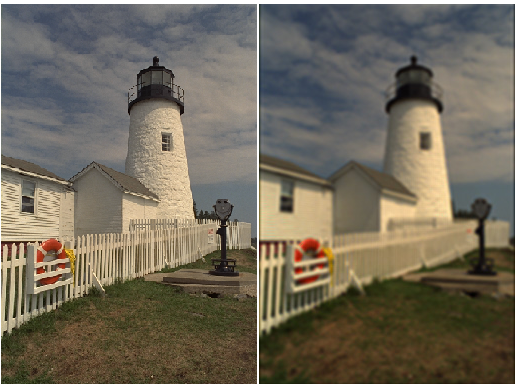
\includegraphics[scale=0.66]{imagenes/blurring}
	\label{blurring}
  \end{center}
\end{figure}

\begin{figure}[h!]
	\caption{A la izquierda, la imagen original. A la derecha, la que presenta <<false color>>.}
	\begin{center}
	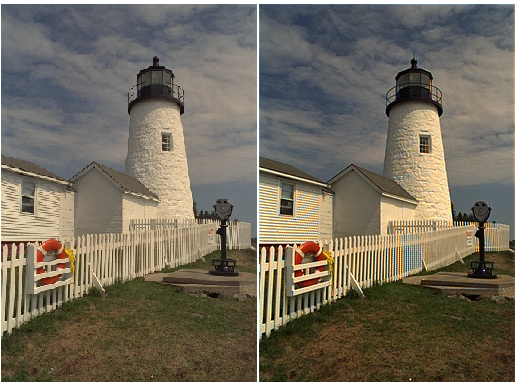
\includegraphics[scale=0.66]{imagenes/false}
	\label{false}
  \end{center}
\end{figure}

\newpage

\begin{figure}[h!]
	\caption{A la izquierda, la imagen original. A la derecha, la que presenta <<zipper>>.}
	\begin{center}
	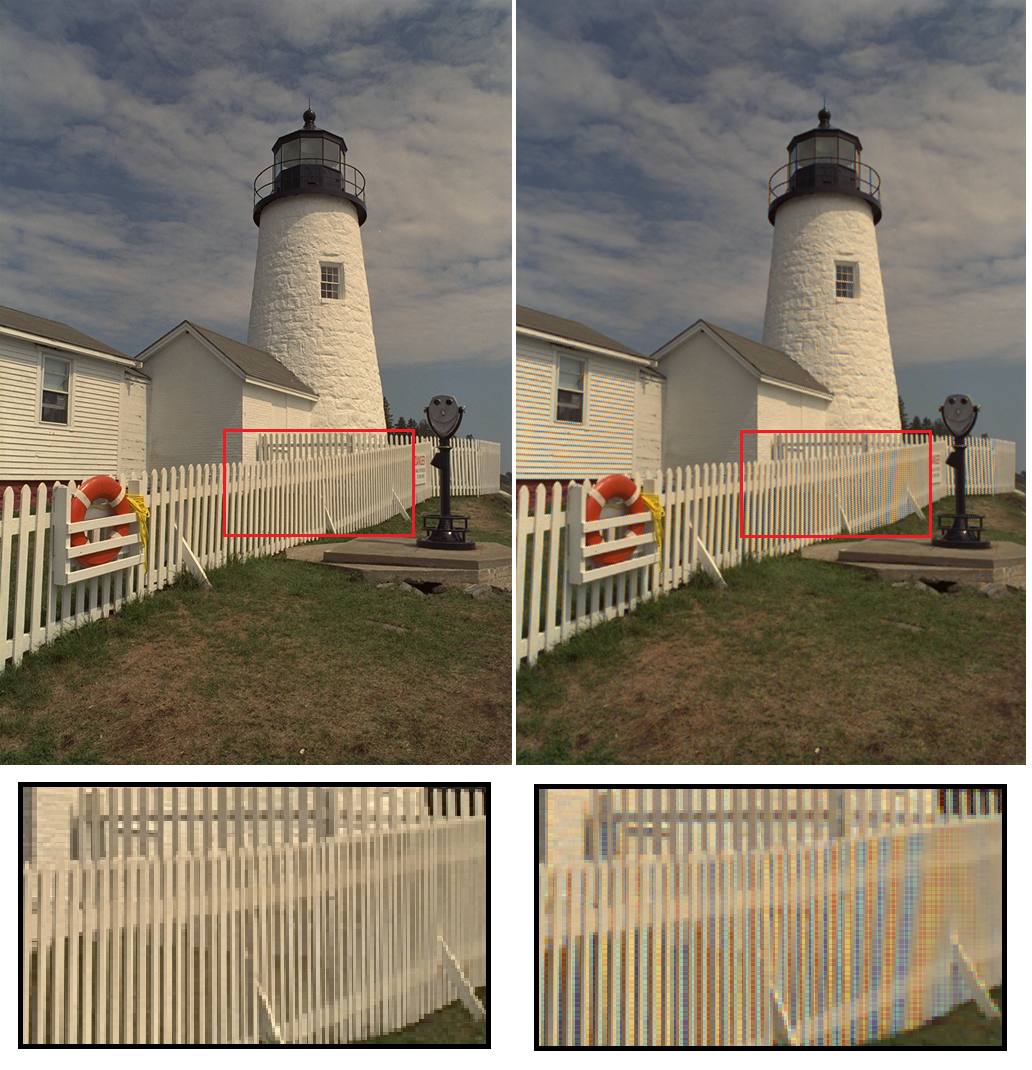
\includegraphics[scale=0.50]{imagenes/zipper}
	\label{zipper}
  \end{center}
\end{figure}

\begin{figure}[h!]
	\caption{A la izquierda, la imagen original. A la derecha, la que presenta <<jaggies>>.}
	\begin{center}
	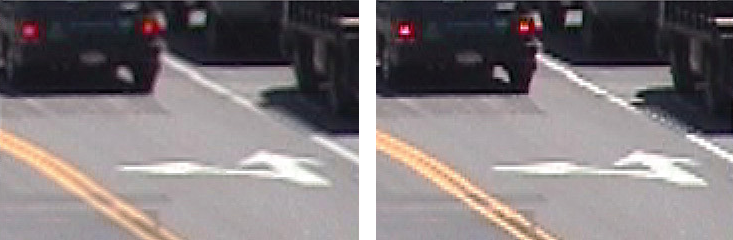
\includegraphics[scale=0.50]{imagenes/jaggies}
	\label{jaggies}
  \end{center}
\end{figure}

\newpage

\begin{figure}[h!]
	\caption{A la izquierda, la imagen original. A la derecha, la que presenta el efecto <<moiré>>.}
	\begin{center}
	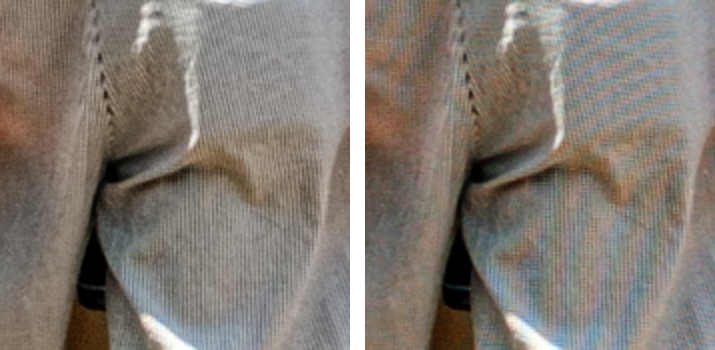
\includegraphics[scale=0.50]{imagenes/moire}
	\label{moire}
  \end{center}
\end{figure}







\textcolor{red}{ESTARÍA BUENO AGREGAR TIPO ANECDÓTICO LOS ARTIFACTS DEL OJO HUMANO (?) PERO NO SÉ EN PRINCIPIO CÓMO MECHARLO ACÁ}





\newpage
\section{Desarrollo}

Dada una \textit{imagen cruda}, los valores que contiene en sus píxeles para cada canal los asumimos reales y ciertos. Por lo tanto, resta averiguar para cada uno de ellos los valores de los dos canales para los cuales dicha información se encuentra ausente.

\subsection{Vecino m\'as cercano}
La implementación más sencilla para la estimación de los canales desconocidos de cada pixel consiste en otorgar a cada canal ``vacío'' el valor real m\'as pr\'oximo que corresponda a dicho color. Este m\'etodo es algor\'itmicamente asequible, pero no tiene en cuenta dos factores: \\
\\

$\triangleright$ Por un lado, al otorgar el valor de un sólo pixel cercano, surge la necesidad de definir arbitrariamente cuál se debe escoger como valor referencial en casos en que un conjunto de pixeles son equidistantes al analizado y no existe un criterio claro acerca de cuál de ellos debe ser considerado el ``más próximo''. Que esta decisión impacte en el resultado de forma inocua o parcial o totalmente nociva dependerá en cierta medida de la fotografía que se esté analizando.

El ejemplo más trivial se encuentra en una imagen monocromática: al ser los valores reales idénticos para todos los pixeles, tomar las magnitudes de cualquier otra posición para cada canal correspondiente no afectará el resultado final. Sin embargo, si consideráramos una imagen formada por columnas alternadas de un pixel de ancho rojas (\#0000FF) y blancas (\#FFFFFF), entonces podríamos analizar cómo sería procesada si se resolviera:

\begin{itemize}
\item \textbf{Caso 1}: 
    Adjudicar:
\begin{itemize}
\item   A los valores nativos verdes: Los valores nativos - rojo y azul - que se encuentren a la derecha y por debajo de su posición.
\item   A los valores nativos azules: El valor verde de la posición inferior y el del rojo  cuya ubicación se encuentra en su diagonal inferior derecha.
\item   A los valores nativos rojos: El valor verde de la posición inferior y el del azul cuya ubicación se encuentra en su diagonal inferior derecha.  
\end{itemize}

\item \textbf{Caso 2}: 
    Adjudicar:
\begin{itemize}
\item   A los valores nativos verdes: Los valores nativos - rojo y azul - que se encuentren a la derecha y por debajo de su posición.
\item   A los valores nativos azules: El valor verde de la posición derecha y el del rojo cuya ubicación se encuentra en su diagonal inferior derecha.
\item   A los valores nativos rojos: El valor verde de la posición derecha y el del azul  cuya ubicación se encuentra en su diagonal inferior derecha.
\end{itemize}

    
\end{itemize}

Los procedimientos y resultados de las experimentaciones realizadas con estos dos criterios se encuentran respectivamente en las Figuras \ref{apxlvecino0}, \ref{apxlvecino1} y \ref{apxlvecino2} para el \textbf{Caso 1} y en las ilustraciones \ref{apxlvecino0}, \ref{apxlvecino1} y \ref{apxlvecinoOTRO2} para el \textbf{Caso 2}.

\begin{figure}[h!]
    \caption{}
    \begin{center}
    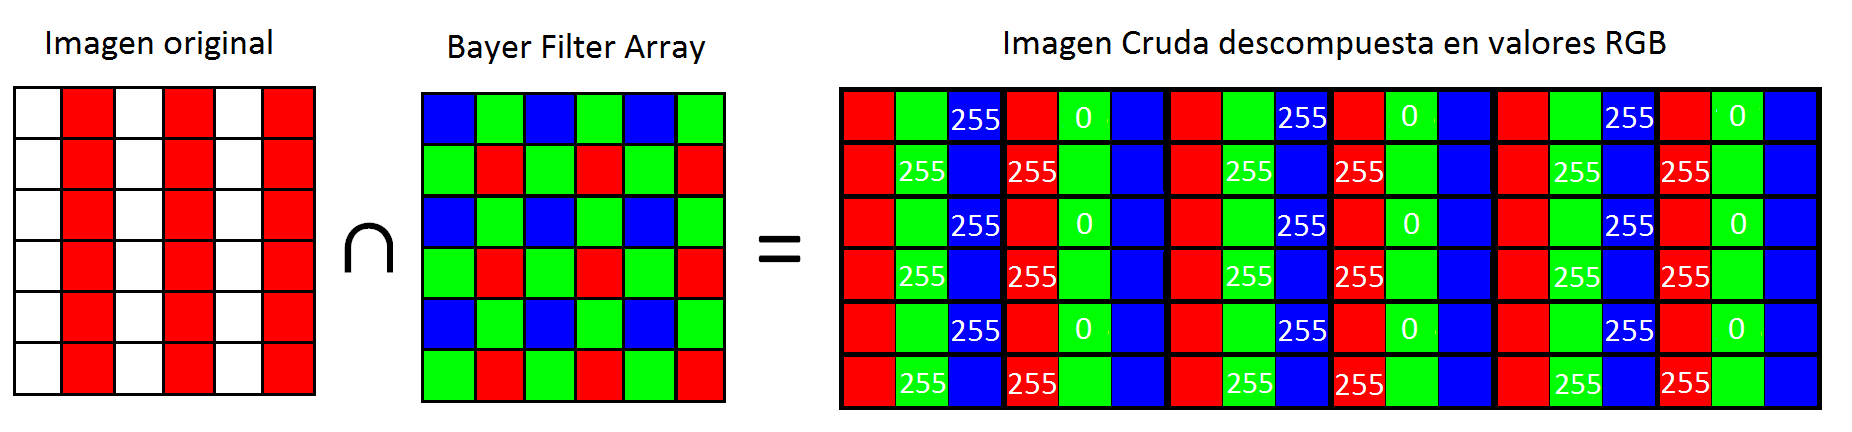
\includegraphics[scale=0.35]{imagenes/apxlvecino0}
    \label{apxlvecino0}
  \end{center}
\end{figure}

\begin{figure}[h!]
    \caption{}
    \begin{center}
    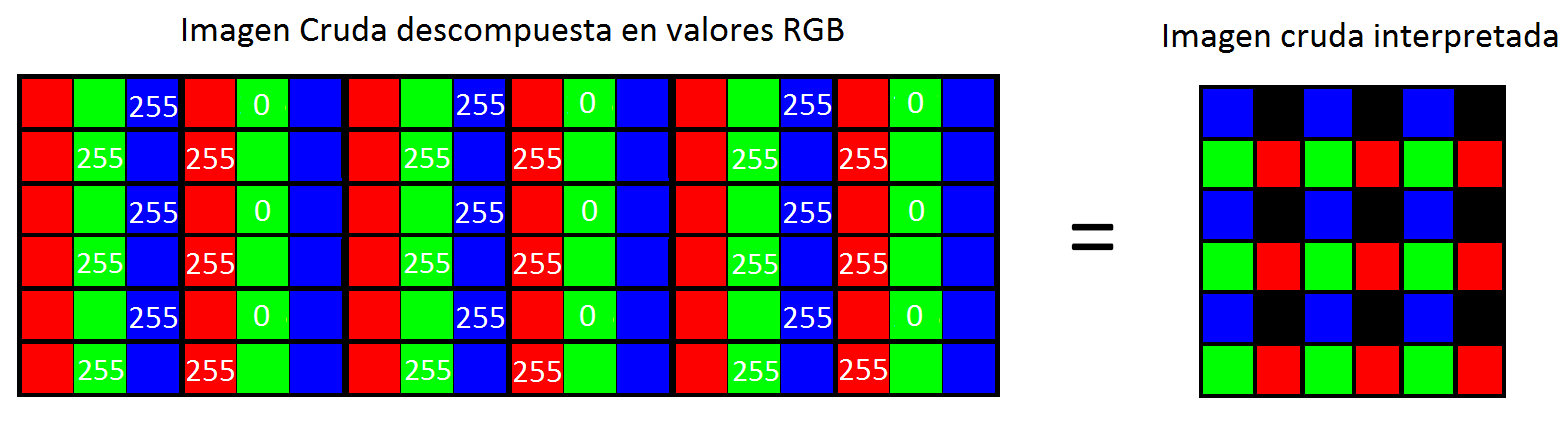
\includegraphics[scale=0.45]{imagenes/apxlvecino1}
    \label{apxlvecino1}
  \end{center}
\end{figure}


\begin{figure}[h!]
    \caption{Valores para todos los canales luego de la interpolación realizada con un algoritmo de ``vecino más cercano'', \textbf{Caso 1}}
    \begin{center}
    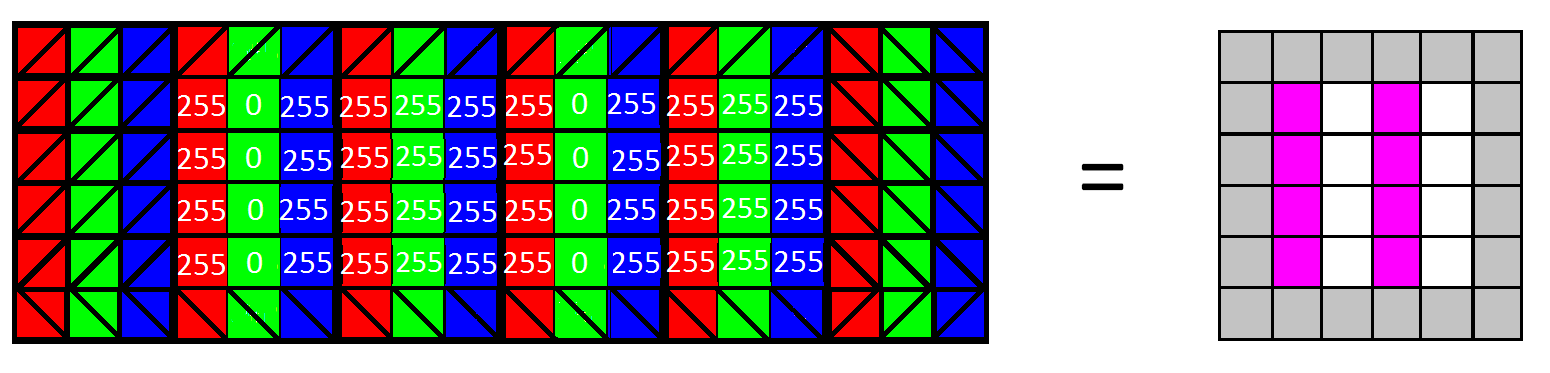
\includegraphics[scale=0.45]{imagenes/apxlvecino2}
    \label{apxlvecino2}
  \end{center}
\end{figure}

\begin{figure}[h!]
    \caption{ Valores para todos los canales luego de la interpolación realizada con un algoritmo de ``vecino más cercano'', \textbf{Caso 2}}
    \begin{center}
    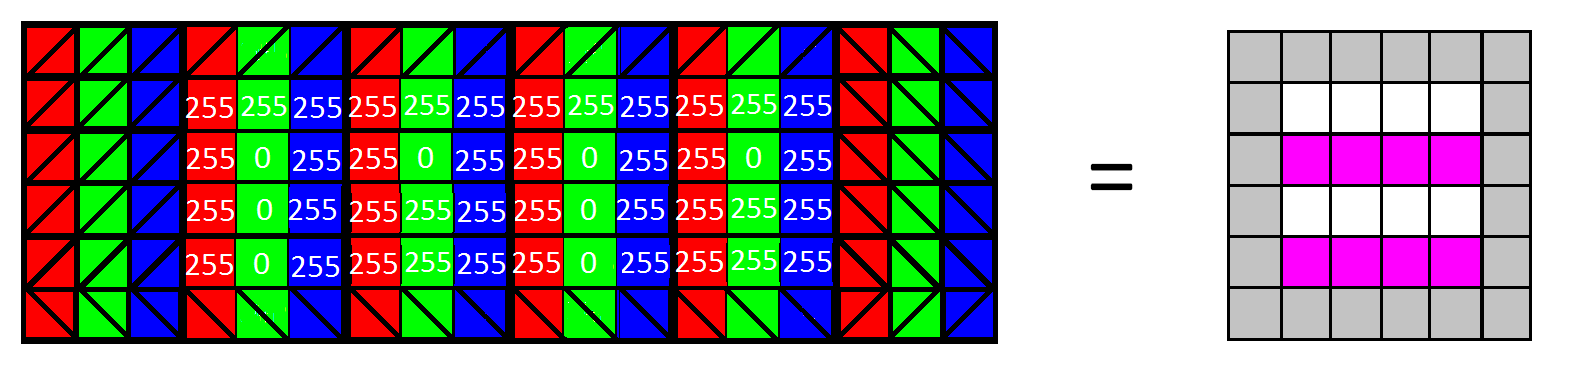
\includegraphics[scale=0.45]{imagenes/apxlvecinoOTRO2}
    \label{apxlvecinoOTRO2}
  \end{center}
\end{figure}

\newpage

Como se ve, en ninguno de los dos casos se logró reconstruir la imagen original, pero sin duda alguna el error en el primer caso fue menor al segundo.\\

El algoritmo planteado evidencia que los resultados proporcionados serán acordes a la imagen que se procesa y a las decisiones arbitrarias que se tomen al implementarlo. \\

Si bien se trata de un ejemplo de alcance limitado, resulta suficiente para ilustrar los potenciales problemas de la aplicación de este algoritmo.\\



$\triangleright$ Por otra parte - y en cierta forma vinculado al ejemplo anterior - este método no especifica ninguna distinción respecto de la forma de proceder en casos de borde o de superficies parejas. \\


\newpage
\subsection*{Decisiones tomadas en el Algoritmo de Vecino M\'as Cercano}

A la hora de formular nuestro algoritmo de Vecino m\'as Cercano nos vimos obligados a determinar aspectos que conciernen al dise\~no del mismo. 

La principal decisi\'on que debimos tomar fue con qu\'e criterio elegir al p\'ixel m\'as cercano cuando no es \'unico (esto ocurre en todos los casos). 

\begin{figure}[h!]
	\caption{}
	\begin{center}
	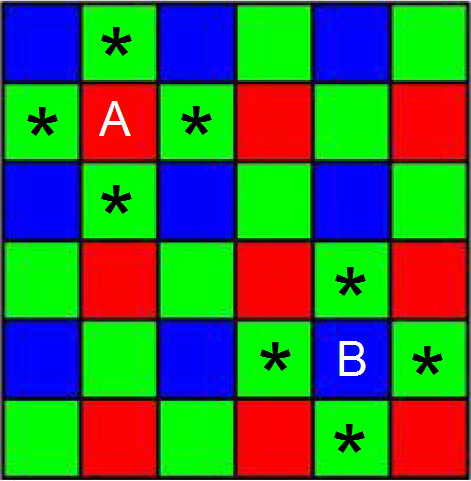
\includegraphics[scale=0.36]{imagenes/vecino1}
	\label{Vecino1}
  \end{center}
\end{figure}

Para determinar el valor del canal verde sobre un p\'ixel definido rojo\emph{(A)} o azul\emph{(B)} tenemos cuatro p\'ixeles a la misma distancia (1) que nos brindan informaci\'on sobre el canal verde. 
\begin{figure}[h!]
	\caption{}
	\begin{center}
	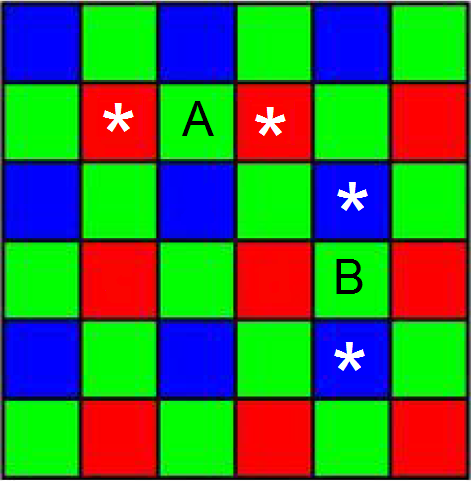
\includegraphics[scale=0.36]{imagenes/vecino2}
	\label{Vecino2}
  \end{center}
\end{figure}

Si nos situamos en un p\'ixel naturalmente verde, tanto para determinar su canal rojo\emph{(A)} como para determinar su canal azul\emph{(B)} sus p\'ixeles m\'as cercanos que nos brindan informaci\'on son dos (a 1 de distancia cada uno). 
\begin{figure}[h!]
	\caption{}
	\begin{center}
	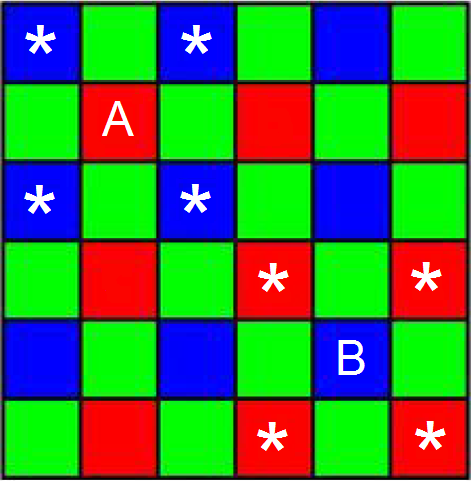
\includegraphics[scale=0.36]{imagenes/vecino3}
	\label{Vecino3}
  \end{center}
\end{figure}

Y por \'ultimo para determinar el valor del canal azul sobre un p\'ixel de origen rojo\emph{(A)} (y viceversa\emph{(B)}) nos encontramos con cuatro p\'ixeles a la misma m\'inima distancia (2) en sus diagonales. \\

Por este motivo, realizamos dos versiones de este algoritmo variando en ellas cu\'al p\'ixel elegir para rellenar el canal verde cuando se est\'a situado sobre un p\'ixel azul o rojo.

En el \emph{\textbf{algoritmo 1}} si se est\'a en un p\'ixel rojo se elige al de arriba y si se est\'a en un p\'ixel azul se elige el de la derecha. En cambio, en el \emph{\textbf{algoritmo 2}} si se est\'a en un p\'ixel rojo se elige al de la izquierda y si se est\'a en un p\'ixel azul se elige al de abajo.

Corrimos ambos algoritmos con diversas fotos, a continuaci\'on se muestran algunos ejemplos que contienen detallado el valor de psnr y ssim para cada imagen respecto de la original.

\begin{figure}[h!]
	\caption{}
	\begin{center}
	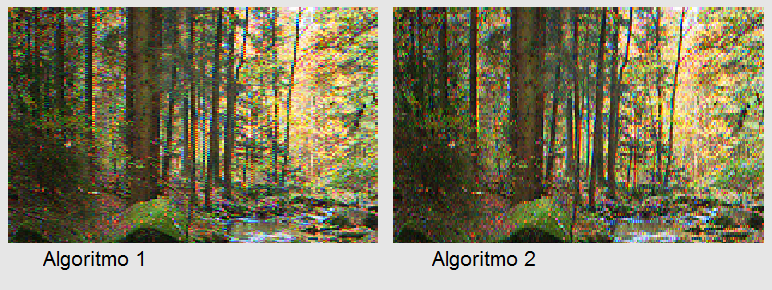
\includegraphics[scale=0.60]{imagenes/Vecino/arbolitos}
	\label{arbolitos}
	
	psnr1 =   14.3119

psnr2 =   14.3533

ssim1 =    0.3819

ssim2 =    0.3856
  \end{center}
\end{figure}

\begin{figure}[h!]
	\caption{}
	\begin{center}
	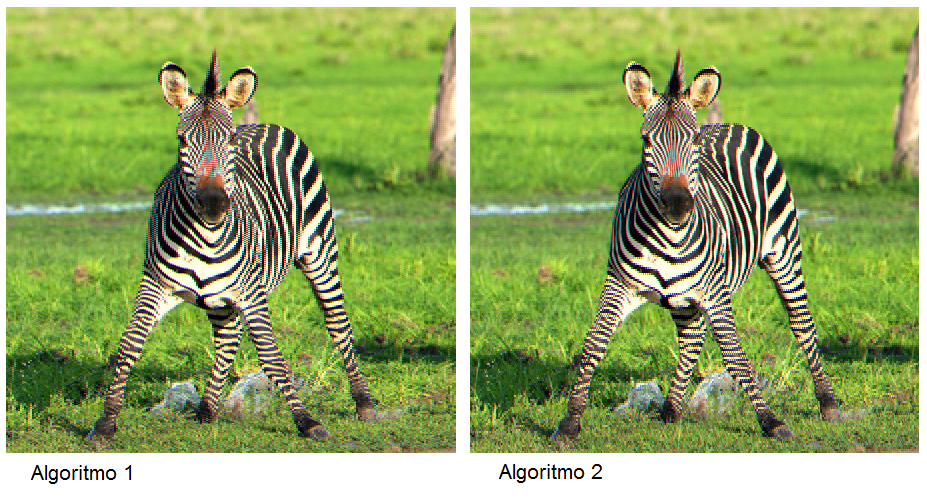
\includegraphics[scale=0.60]{imagenes/Vecino/zebraCara}
	\label{zebraCara}
	
	psnr1 =   19.8295

psnr2 =   20.0706

ssim1 =    0.8806

ssim2 =    0.8841
  \end{center}
\end{figure}

\newpage
\begin{figure}[h!]
	\caption{}
	\begin{center}
	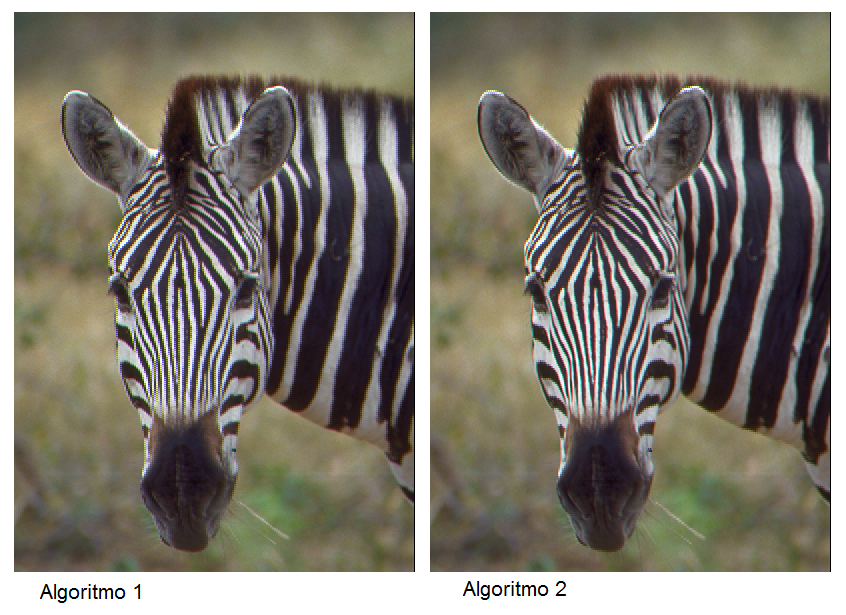
\includegraphics[scale=0.60]{imagenes/Vecino/zebra}
	\label{Zebra}
	
	psnr1 =   21.1167

psnr2 =   21.3368

ssim1 =    0.8374

ssim2 =    0.8417
  \end{center}
\end{figure}


\begin{figure}[h!]
	\caption{}
	\begin{center}
	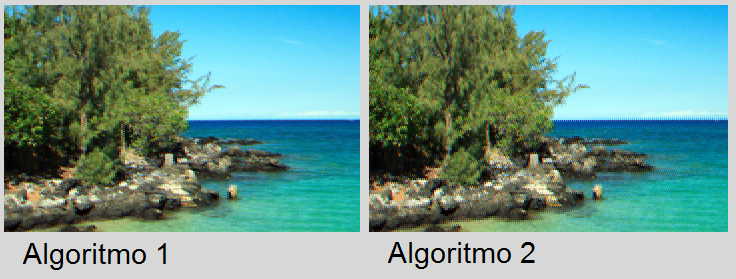
\includegraphics[scale=0.06]{imagenes/Vecino/hawaiicmp}
	\label{Zebra}
	
	psnr1 =   23.2721

psnr2 =   23.2371

ssim1 =    0.8560

ssim2 =    0.8553
  \end{center}
\end{figure}

\newpage

\begin{figure}[h!]
	\caption{}
	\begin{center}
	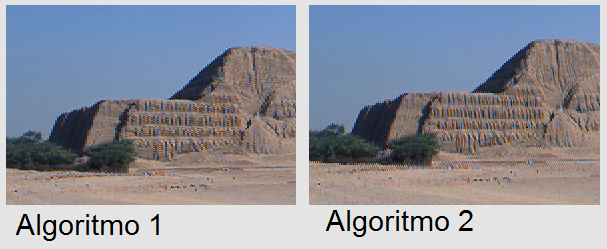
\includegraphics[scale=0.06]{imagenes/Vecino/piramides3cmp}
	\label{Zebra}
	
	psnr1 =   23.8518

psnr2 =   23.8270

ssim1 =    0.7514

ssim2 =    0.7515
  \end{center}
\end{figure}

\begin{figure}[h!]
	\caption{}
	\begin{center}
	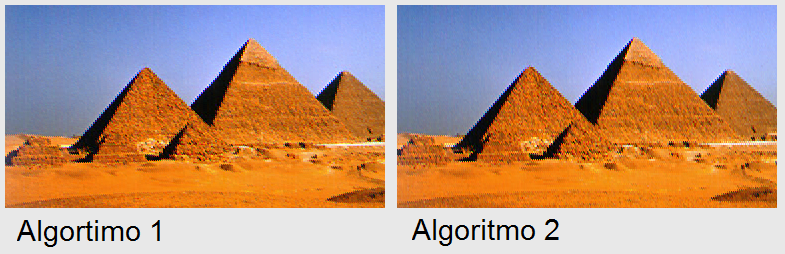
\includegraphics[scale=0.70]{imagenes/Vecino/piramides2cmp}
	\label{Zebra}
	
	psnr1 =   21.7691

psnr2 =   21.7494

ssim1 =    0.9508

ssim2 =    0.9506
  \end{center}
\end{figure}




Se puede apreciar que el Algoritmo 1 es capaz de delimitar mejor bordes que poseen rayas en forma horizontal, en cambio el Algoritmo 2 le da una mejor definici\'on a los bordes verticales. Dada la forma de la implementaci\'on, las anomal\'ias observadas en las imagenes cobran sentido.\\


Debido a que no se puede establecer con un criterio cu\'al es m\'as correcta que la otra, ya que la veracidad de la imagen obtenida var\'ia depende la imagen inicial y su estructura. Nosotros optamos por utilizar el \emph{\textbf{Algoritmo 1}}.\\

\textit{Se adjuntan las im\'agenes en su tama\~no original.}

\newpage
\subsection{Interpolaci\'on Bilineal}

La interpolación bilineal es una composición de interpolaciones lineales en dos direcciones diferentes. Este método desmerece el caracter arbitrario de asignación de un canal a partir del valor más próximo para el mismo y propone que el resultado final sea calculado teniendo en cuenta y promediando todos los valores cercanos sin priorizar ninguno de ellos. \\

Como la estructura del filtro Bayer sólo asegura para los p\'ixels nativamente azules o rojos tener todas sus posiciones vecinas netamente verdes, aquel es el único caso en que el cálculo de un canal se reduce a computar el promedio de los valores superior, inferior, derecho e izquierdo al espacio que se quiere interpolar.\\

Sin embargo, si se quisiera obtener el valor de azul o rojo que correspondería asignar a un p\'ixel nativamente verde, el entramado de Bayer obligaría a estimarlo a partir de sus dos valores m\'as cercanos ubicados a la derecha e izquierda o arriba y abajo dependiendo de la ubicaci\'on del p\'ixel. \\

Por otro lado, los valores del canal azul para un p\'ixel rojo (y los del canal rojo para un p\'ixel azul) se calcularían tomando en cuenta las cuatro posiciones diagonales a la analizada. Este proceso no se realizar\'ia simplemente tomando el promedio de sus cuatro diagonales sino que requeriría tomar dos p\'ixels cercanos que pertenezcan a la misma fila o columna, cuyo canal real sea el verde, calcular sus valores de azul/rojo promediando los de las casillas nativas azules/rojas más próximas y posteriormente realizar un nuevo promedio entre los valores resultantes.\\

Tomando como referencia la ilustración \ref{bilineal} se puede ver que el cálculo recien descripto equivale a calcular el valor en el canal rojo para el p\'ixel x. Lo cual consistir\'ia en: 

\begin{itemize}
 
\item Hacer el promedio entre \textit{a y b} y luego, ubicar ese valor para el canal rojo para el p\'ixel ubicado arriba de x.

\item Hacer el promedio entre \textit{c y d} y luego, ubicar ese valor para el canal rojo para el p\'ixel ubicado debajo de x.

\item Una vez obtenidos estos dos valores, promediarlos y ubicarlos en el canal rojo de x.\\
\end{itemize}
Llegando as\'i a que realizar este c\'alculo es equivalente a realizar el promedio entre los valores de sus diagonales:

\[
 \frac{\frac{a+b}{2} + \frac{c+d}{2}}{2} = \frac{a+b+c+d}{4}
\]

\begin{figure}[h!]
	\caption{}
	\begin{center}
	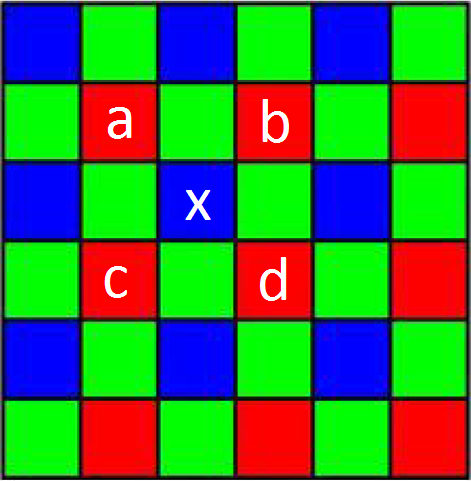
\includegraphics[scale=0.36]{imagenes/bilineal}
	\label{bilineal}
  \end{center}
\end{figure}

\newpage
\subsection{Interpolaciones Direccionales}
Se trata de una gran cantidad de métodos que buscan comenzar a resolver el problema de demosaicing realizando inicialmente una interpolación en una dirección y combinando con algún criterio determinado el resultado estimado con el obtenido de una aproximación realizada en otra dirección.\\

La implementación de este tipo de métodos exige tomar al menos dos decisiones de peso que distinguirán a unos de otros:\\

\begin{itemize}
    \item De qué forma se realizarán las interpolaciones (en qué direcciones y mediante qué mecanismo de interpolación)
    \item Con qué criterio y consideraciones combinar la información proporcionada por las direcciones escogidas.
\end{itemize}

Para escoger alguna opción apropiada corresponde analizar las características del Color Filter Array con el que se va a trabajar, puesto que no todas las direcciones van a aportar en la totalidad de los casos la misma información.

En cuanto a la combinación de los resultados de las distintas interpolaciones, es conveniente tener presente que el promedio de los mismos no es siempre una buena opción. Por ejemplo, supongamos que se analiza una imagen que presenta en un sector las características observables en la Imagen original de la ilustración \ref{apxl1}.


\begin{figure}[h!]
	\caption{}
	\begin{center}
	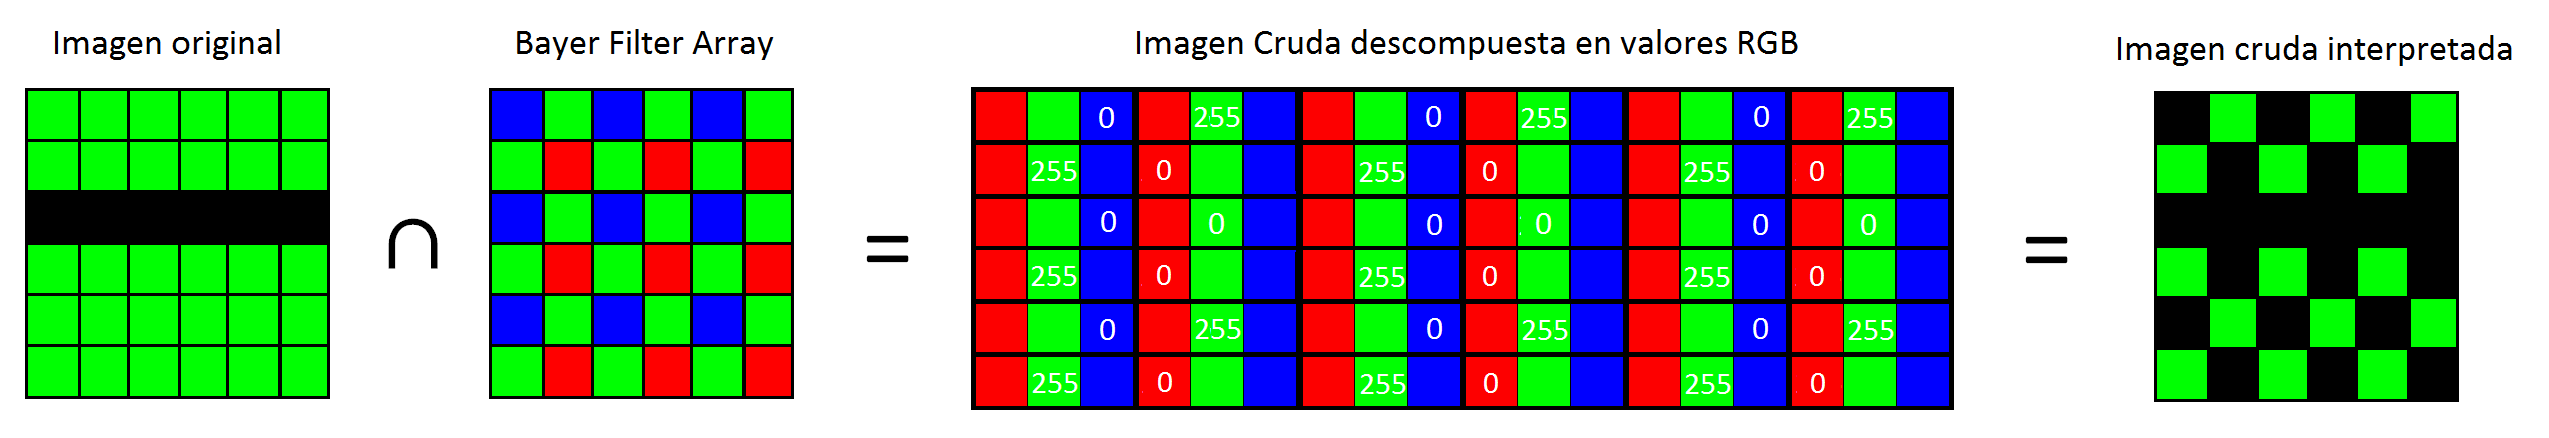
\includegraphics[scale=0.23]{imagenes/apxl1}
	\label{apxl1}
  \end{center}
\end{figure}

En dicha figura se analiza la información de la misma que sería captada por los fotosensores respondiendo al Bayer Filter Array. 

En el esquema \ref{apxl2} se puede observar que para varios p\'ixeles la interpolación horizontal retorna valores distintos a la realizada verticalmente (esto tiene sentido, pues se trata de un área homogénea atravesada por una fila de distinto color).

El resultado de empleo del promedio como estrategia de nivelacion de dichos valores queda expuesto en la Figura \ref{apxl3}, en la cual se puede observar el causante del artifact ``zipping'', producto de un algoritmo indiferente ante los cambios de color abruptos.\\

\begin{figure}[h!]
	\caption{}
	\begin{center}
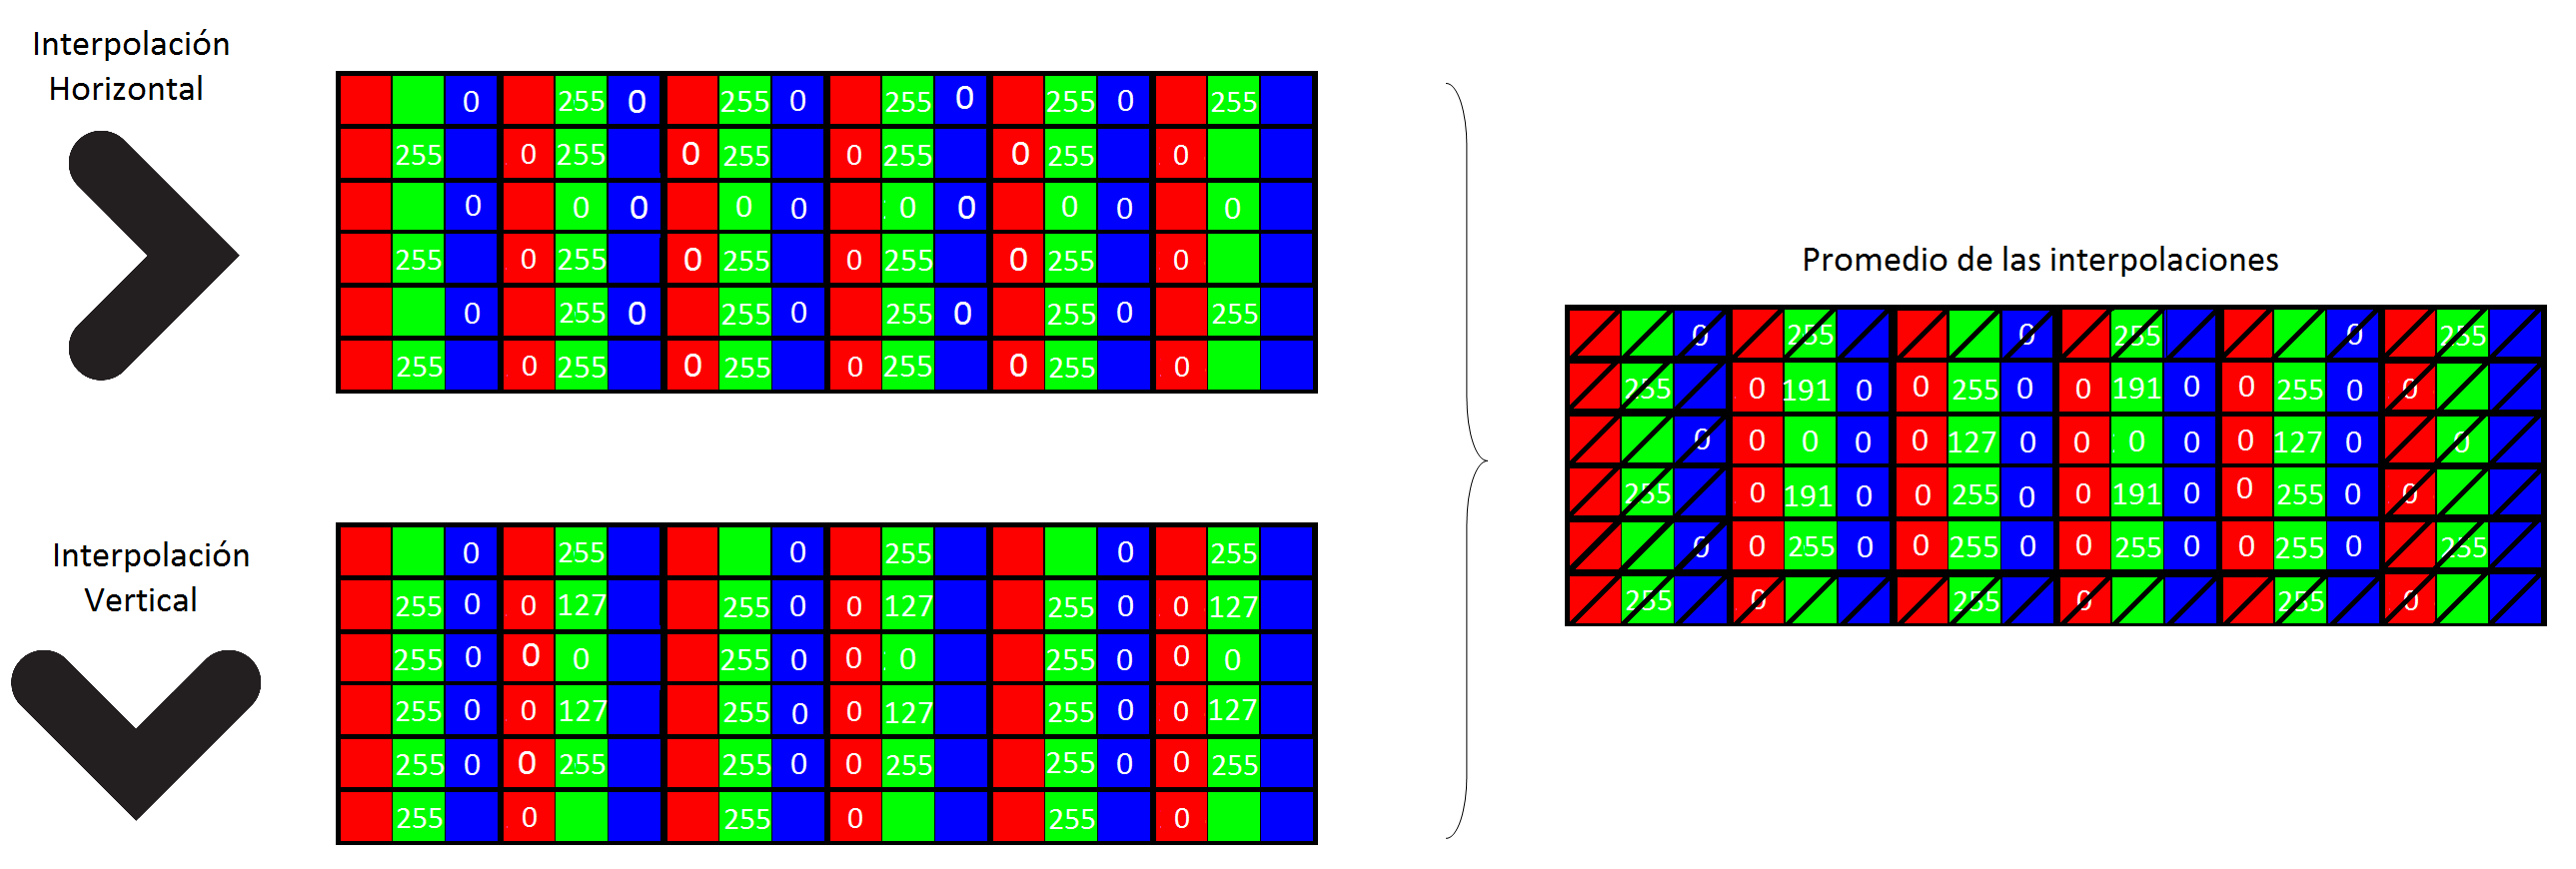
\includegraphics[scale=0.26]{imagenes/apxl2}
	\label{apxl2}
  \end{center}
\end{figure}

\begin{figure}[h!]
	\caption{}
	\begin{center}
	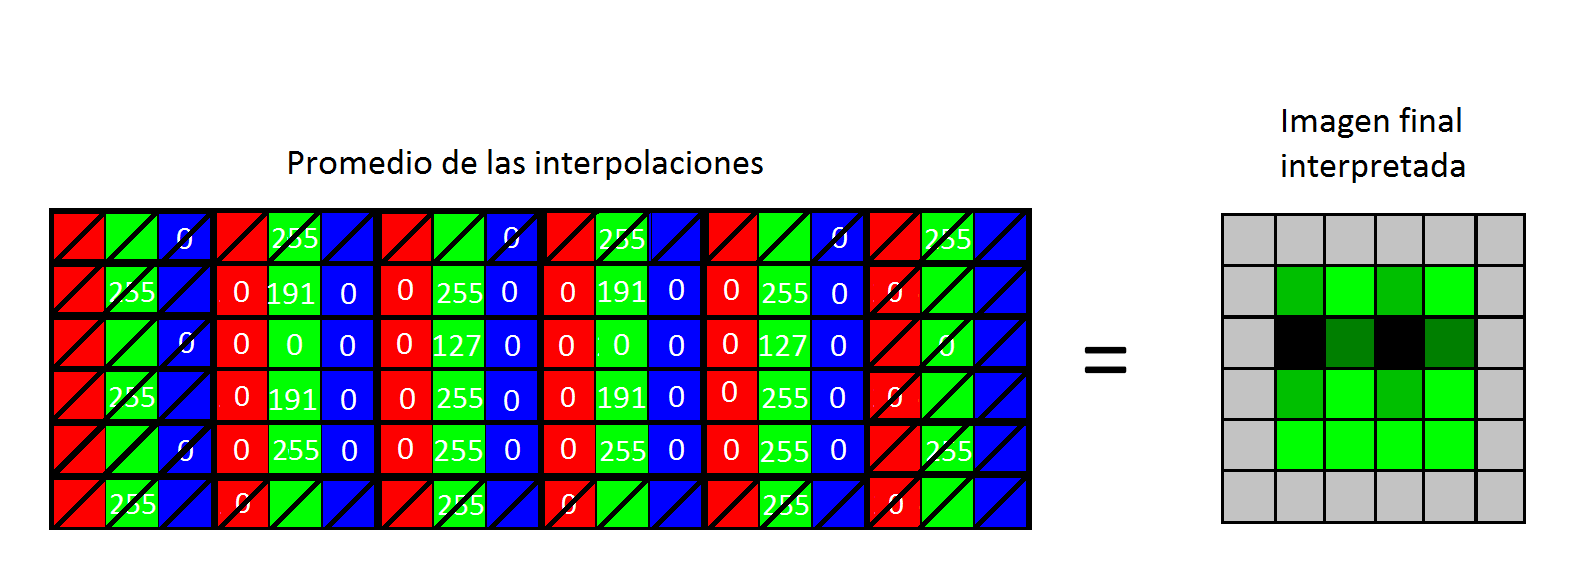
\includegraphics[scale=0.36]{imagenes/apxl3}
	\label{apxl3}
  \end{center}
\end{figure}

\newpage
Ciertamente esto no es lo esperado y existen mecanismos que permiten corregir este error. Uno de ellos consiste en calcular el gradiente del color para utilizarlo al combinar los resultados, de modo tal que si el mismo fuera de gran magnitud (es decir, la variación del color es considerable) entonces el peso que debe tener el valor calculado en el resultado final debería ser menor a aquel que fue calculado en una dirección cuyo gradiente fuera menor (es decir, que se tratara de una superficie más cromáticamente homogénea).



\pagebreak

\newpage
\subsection{Splines}
\subsubsection*{Generación de los Splines}
\textcolor{red}{No se si estan de acuerdo, pero no me pareceria mal dividir un poco la intro teórica en este TP, y hablar acá de por qué no usamos Lagrange. Si no les parece da igual, acá se puede hacer referencia a eso. Y listo (es lo que voy a dejar escrito ahora) pero hay que meditar qué queda mejor.}

\textcolor{blue}{Hablar de todos sus tipos\\
Decir que bilineal y poner 0.5 queda igual (o casi igual je), usar psnr.\\
Y ver cual vamos a dejar\\
Y que usamos NATURALES}

Yendo un paso más allá de la interpolación bilineal, podemos preguntarnos qué otros métodos existen que nos permitan obtener mejores resultados. Una buena primera idea sería analizar qué sucede con los Splines. \\

Los Splines (o trazadores cúbicos) son un tipo particular de interpoladores fragmentarios: funciones partidas que interpolan a través de polinomios un conjunto de puntos. En el caso de los Splines, se interpola entre dos puntos mediante un polinomio cúbico.\\

Como fue explicado anteriormente, los Splines son una opción muy buena a la hora de interpolar funciones: en el análisis realizado contra el Polinomio de Lagrange pudimos observar que este último puede llegar a ser excesivamente malo en ciertos casos. Considerando la superioridad de los Splines, entonces, nos propusimos encontrar un algoritmo que los utilice para conseguir buenas interpolaciones que generen imágenes de calidad superior a la hora de realizar el demosaicing.\\

Conseguir el Spline interpolador de una función $f$ dado un conjunto de puntos \{\(X_0, ..., X_n\)\} y sus respectivos valores de $f(x_j)$ consiste en resolver un sistema \(Ax = b\) que nos permita encontrar los 4 coeficientes de cada uno de los $n-1$ polinomios que lo conformen. Siguiendo la lógica presentada en \textbf{[3]}, donde se despeja el coeficiente que acompaña al término de grado 2 en cada polinomio, se puede llegar a ver que $A$ resulta ser una matriz tridiagonal de $(n+1)\times(n+1)$ que posee el siguiente aspecto (trabajando con splines naturales): \\

\[
A = \left(
\begin{array}{cccccccccc}
1 &  &  &  &  &  &  & &  & \\
h_0 & 2\cdot(h_0+h_1) & h_1 &   & & & & &  & \\
 & h_1 & 2\cdot(h_1+h_2) & h_2 & & & & &  & \\
 &  &  & \ddots &  &  &  &  &  &  \\
 &  &  &  & h_j & 2\cdot(h_j+h_{j+1}) & h_{j+1} & &  & \\
 &  &  &  &  &  & \ddots &  &  &  \\
 &  &  &  &  & & & h_{n-2} & 2\cdot(h_{n-2}+h_{n-1}) &h_{n-1}\\
 &  &  &  &  &  &  &  &  & 1
\end{array}
\right)
\]

\bigskip
\noindent Donde $h_j$ es igual a la distancia entre los puntos $X_j$ y $X_{j+1}$. \\
Mientras tanto, $b$ será un vector de la forma:

\[
b_i =
\begin{cases}
0 & i = 0 \lor i = n \\
\frac{3\cdot(f(x_{i+1})-f(x_i))}{h_i} - \frac{3\cdot(f(x_i)-f(x_{i-1}))}{h_{i-1}} & 1 \leq i \leq n-1
\end{cases}
\]

\bigskip
Para nuestro problema en particular, vamos a considerar las funciones a interpolar como el valor de un canal de RGB en alguna porción de la imagen. Dada la fisonomía del Bayer Filter Array, puede observarse con facilidad que, tomando una fila o una columna cualesquiera, la distancia que hay entre dos píxeles del mismo color es de 2 unidades (es decir, para un pixel azul en la posición $j$ de una fila, el siguiente pixel azul se va a encontrar en la posición $j+2$). Esto incluso aplica a si tomamos diagonales (no las que contienen exclusivamente verde, aunque dicho caso no nos es de interés ya que no se interpolaría el verde sobre la misma). \\
Por esta razón, podemos reemplazar $h_j$ por 2, para todo $j$, y obtener: \\

\[
A = \left(
\begin{array}{cccccccccc}
1 &  &  &  &  &  &  & &  & \\
2 & 8 & 2 &   & & & & &  & \\
 &  & \ddots &  &  &  &  &  &  &  \\
 &  &  &  & 2 & 8 & 2 & &  & \\
 &  &  &  &  &  & \ddots &  &  &  \\
 &  &  &  &  & & & 2 & 8 & 2\\
 &  &  &  &  &  &  &  &  & 1
\end{array}
\right)
\]

\bigskip

\[
b_i =
\begin{cases}
0 & i = 0 \lor i = n \\
\frac{3\cdot(f(x_{i+1})-2\cdot f(x_i)+f(x_{i-1}))}{2} & 1 \leq i \leq n-1
\end{cases}
\]

\bigskip
Este sistema tiene la particularidad de que $A$ es estrictamente diagonal dominante, y por lo tanto va a tener solución única, con lo cual sabemos que el método interpolador funcionará correctamente. \\

Una vez resuelto el mismo, sólo queda despejar los coeficientes principales y el de grado 1 de cada polinomio. El algoritmo en su totalidad se describe a continuación:

\IncMargin{1em}
\begin{algorithm}[h!]
\NoCaptionOfAlgo
\caption{Algoritmo generar_spline}
\SetKwInOut{Input}{input}\SetKwInOut{Output}{output}

\Input{Vector F}
\Output{Vector S}
\bigskip

n = size(F)\\
Matriz A(n)\\
Vector S($4\cdot(n-1)$)\\
\bigskip
A($0,0$) = 1\\
A($n-1,n-1$) = 1\\
b($0$) = $0$\\
b($n-1$) = $0$\\
\bigskip
\For{cada fila i de la matriz A}{
A($i,i-1$) = 2\\
A($i,i$) = 8\\
A($i,i+1$) = 2\\
b($i$) = $\frac{3\cdot(F(x_{i+1})-2\cdot F(x_i)+F(x_{i-1}))}{2}$
}
\bigskip
Resolver el sistema $Ax=b$ y guardarlo en el vector $sol$\\
\bigskip
\For{cada elemento i del vector sol}{
S($i$) = F($i$)\\
S($(i \cdot 4)+1$) = $\frac{f(x_{i+1})-f(x_i)}{2}-\frac{2\cdot sol(i+1)+ 4\cdot sol(i)}{3}$\\
S($(i \cdot 4)+2$) = $sol(i)$\\
S($(i \cdot 4)+3$) = $\frac{sol(i+1)-sol(i)}{6}$\\
}
\bigskip
Retornar S
\end{algorithm}\DecMargin{1em}

\bigskip
Notar que $F$ representa un vector que contiene los valores de $f(X_j)$ que queremos interpolar. Por otro lado, el conjunto de puntos \{\(X_0, ..., X_n\)\} está implícito, ya que, como la distancia entre ellos es siempre 2, no es necesario saber su valor para realizar la interpolación: los consideramos enumerados de 0 a $n$. \\
\indent Por su parte, $S$ es un vector que contiene los cuatro coeficientes de cada polinomio, de corrido, ordenados de término independiente a coeficiente principal. \\

Creemos importante comentar acerca de la estructura elegida para las matrices utilizadas: como las matrices que resuelven el problema de la interpolación son siempre matrices tridiagonales, nos pareció una buena idea aprovechar el hecho de que son esparsas para poder trabajar con ellas más eficientemente en términos de memoria y complejidad algorítmica. Para lograr dicho objetivo, procedimos a reutilizar, haciendo algunas modificaciones menores, los algoritmos utilizados en el primer Trabajo Práctico.\\
\indent La estructura elegida, entonces, es un simple vector de vectores, que sólo almacena 4 columnas: las 3 diagonales y el vector resultado. \\

Ya generado el Spline, sólo resta evaluar los puntos que nos interesen para conseguir una estimación de $f$ en los mismos. Para ello, primero se localiza el polinomio cúbico $S_j$ correspondiente en el vector $S$ generado (de acuerdo al intervalo que pertenezca el $X_i$ que se quiere estimar) y se resuelve:

\[f(X_i) \approx a+b\cdot (X_i - X_j)+c \cdot (X_i - X_j)^{2} + d \cdot (X_i - X_j)^{3}\]

\bigskip
Donde $a, b, c$ y $d$ son los coeficientes conseguidos a través del algoritmo \texttt{generar_spline}, y $X_j$ es el valor del punto que se corresponde con el polinomio $S_j$ a utilizar. \\
\indent El algoritmo que resuelve este problema fue implementado de la siguiente manera:

\IncMargin{1em}
\begin{algorithm}[h!]
\NoCaptionOfAlgo
\caption{Algoritmo evaluar}
\SetKwInOut{Input}{input}\SetKwInOut{Output}{output}

\Input{Vector S, Int x}
\Output{Double y}
\bigskip

Int j = $\lfloor \frac{x}{2} \rfloor$ \\
Int i = $4 \cdot j$ \\
\bigskip
Double a = S($i$)\\
Double b = S($i+1$)\\
Double c = S($i+2$)\\
Double d = S($i+3$)\\
\bigskip
j = $2 \cdot j$\\
\bigskip
Retornar $a+b\cdot (x - j)+c \cdot (x - j)^{2} + d \cdot (x - j)^{3}$
\end{algorithm}\DecMargin{1em}

\bigskip
\textcolor{red}{Ver de explicar un poco mejor el tema de las cuentas con los indices\\}
Vale la pena aclarar que el algoritmo recibe como input un entero ya que cada uno de nuestros $X_i$ es un pixel, y no tendría sentido trabajar con fracciones de los mismos. \\

\subsubsection*{Aplicación de Splines al problema de demosaicing}

Una vez resuelto el problema de la implementación de los algoritmos que generan el spline e interpolan valores en el mismo, el siguiente paso fue pensar c\'omo aplicarlo al problema que nos concierne: el \textit{demosaicing} de imágenes. Diversos métodos fueron considerados y estudiados, y serán presentados a continuación. \\
\pagebreak
\begin{figure}[h!]
	\caption{cómo se realiza la interpolación}
	\begin{center}
	    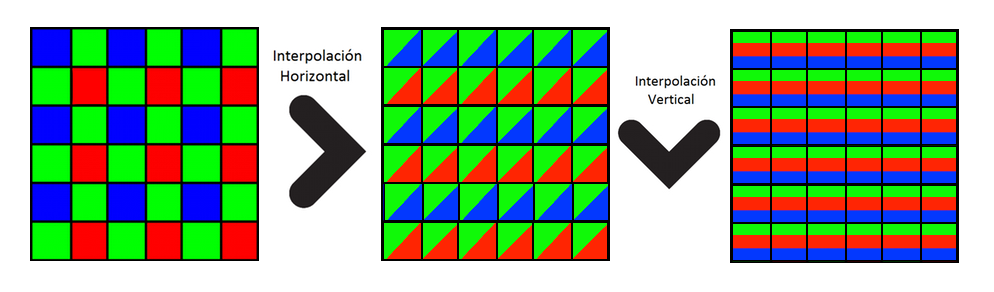
\includegraphics[scale=0.47]{imagenes/Splines/splines1.png}
	\end{center}
	\label{splines1}
\end{figure}

El primer acercamiento que tuvimos con Splines fue simple: para cada pixel, interpolar su fila y su columna (por completo) para los canales faltantes, y asignarle el promedio entre ambos valores obtenidos. \\
Este método aparenta ser muy similar a la interpolación bilineal, donde se asigna el promedio de los valores de sus vecinos, razón por la cual decidimos comparar cualitativamente los outputs de ambos algoritmos:
\begin{itemize}
\item A simple vista, las imágenes son prácticamente idénticas para ambos métodos. Las diferencias son demasiado mínimas como para ser realmente apreciadas. La versión con splines mostró una mayor presencia de artifacts (principalmente \textit{false colors}) pero no muy notable.
\item Objetivamente, las mediciones de PSNR arrojaron valores sorpresivamente distintos (alrededor de 1 punto de diferencia), favoreciendo a la interpolación bilineal.
\end{itemize}

\begin{figure}[h!]
	\begin{center}
	    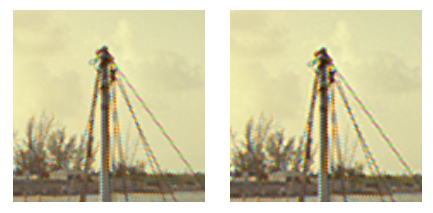
\includegraphics[scale=0.47]{imagenes/Splines/RecortesSplines/promedio/barcos.png}\\
	    PSNR: 28.5901 \ \ \ \ \ \ \ \ \ \ \ \ \ PSNR: 27.6018
	\end{center}
	\begin{center}
	    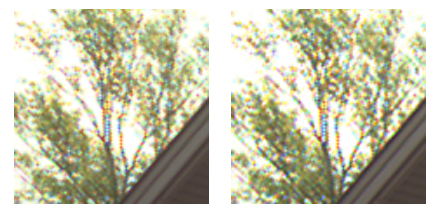
\includegraphics[scale=0.47]{imagenes/Splines/RecortesSplines/promedio/arbol.png}\\
	    PSNR: 27.4478 \ \ \ \ \ \ \ \ \ \ \ \ \ PSNR: 26.154
	\end{center}
	\caption{Interpolación bilineal (izquierda), y mediante esta implementación de Splines (derecha)}
	\label{splines2}
\end{figure}

Respecto al tiempo de ejecución de ambos algoritmos, \textcolor{red}{MEDIR TIEMPOS POR SSH\\}

En vista de estos resultados, decidimos descartar (o mejor dicho, intentar mejorar) el algoritmo mediante Splines, ya que ni en tiempo ni en calidad lo encontramos superior que los métodos anteriores.\\

El primer aspecto con el que decidimos experimentar fue la manera de combinar la información obtenida a través de las interpolaciones. En el caso anterior, simplemente realizábamos el promedio de los valores obtenidos al interpolar una fila y una columna. Sin embargo, este acercamiento no es siempre bueno, ya que puede traer resultados no deseados en los bordes. Es por esta razón que decidimos proponer una idea más sofisticada, detallada brevemente en la sección de interpolación bilineal: el uso del gradiente. \\

A modo de ejemplo, la derivada horizontal en el canal verde del pixel puede estimarse de la siguiente manera:
\[|\partial_xG(x,y)| \approx |G(x-1,y) - G(x+1,y)|\]


Y, análogamente, la vertical:
\[|\partial_yG(x,y)| \approx |G(x,y-1) - G(x,y+1)|\]


Utilizando este concepto, modificamos nuestro algoritmo para que, en lugar de combinar la información obtenida mediante el promedio, haga lo siguiente:

\begin{itemize}
\item Interpolar por filas
\item Al realizar la interpolación por columnas, para los pixeles rojos y azules tenemos ahora dos valores posibles de verde. Comparamos los valores de las derivadas horizontal y vertical para el color verde:
\begin{itemize}
\item Si la derivada horizontal es mayor que la vertical, entonces le asignamos el valor de verde dado por la interpolación de la columna
\item Si la derivada vertical es mayor que la horizontal, entonces le asignamos el valor de verde dado por la interpolación de la fila
\end{itemize}
\end{itemize}

El algoritmo que resuelve esto fue implementado de la siguiente manera:
\begin{algorithm}[h!]
\NoCaptionOfAlgo
\caption{Algoritmo spline_der}
\For{cada fila de la imagen}{
\eIf{la fila es par}{
Generar el spline de toda la fila para el canal azul e interpolar para los píxeles verdes \\
Generar el spline de toda la fila para el canal verde e interpolar para los píxeles azules \\
}{
Generar el spline de toda la fila para el canal rojo e interpolar para los píxeles verdes \\
Generar el spline de toda la fila para el canal verde e interpolar para los píxeles rojos \\
}
}
\bigskip
\For{cada columna de la imagen}{
\eIf{la columna es par}{
Generar el spline de toda la columna para el canal rojo e interpolar para los píxeles azules \\
Generar el spline de toda la columna para el canal azul e interpolar para los píxeles verdes \\
\If{$\partial_xG > \partial_yG$}{
Generar el spline de toda la columna para el canal verde e interpolar para los píxeles azules, reemplazando el valor que había sido asignado en el primer ciclo
}
}{
Generar el spline de toda la columna para el canal azul e interpolar para los píxeles rojos \\
Generar el spline de toda la columna para el canal rojo e interpolar para los píxeles verdes \\
\If{$\partial_xG > \partial_yG$}{
Generar el spline de toda la columna para el canal verde e interpolar para los píxeles rojos, reemplazando el valor que había sido asignado en el primer ciclo
}
}
}
\end{algorithm}

\bigskip

Aplicando este método, pudimos observar mejoras en varios de los bordes de nuestras imágenes: los mismos ahora son más suaves, eliminando casi por completo la presencia de varios artifacts, como por ejemplo zipper.\\
\indent Sin embargo, también hubo algunos aspectos en los cuales la imagen final empeoró: algunas de las lineas más finas mostraron \textit{false colors}, muchas veces con la presencia de algunos píxeles de colores muy fuertes.\\

Respecto a las mediciones de calidad objetivas, los resultados arrojados por PSNR fueron totalmente inesperados: a pesar de ser una diferencia muy chica, PSNR siempre fue superior para la imagen procesada con el método del promedio. Creemos que esto puede deberse a la anormalidad de los colores para ciertos píxeles mencionada en el párrafo anterior, ya que PSNR mide cuánto ``ruido'' hay entre la imagen original y la procesada. \\

De todas maneras, consideramos al método de Splines pesados mediante las derivadas como superior al del promedio, ya que, a la vista, es más notorio que los bordes sean suaves, a que haya algunos pocos píxeles dispersos con colores no muy fieles. \\

Respecto al tiempo de cómputo, \textcolor{red}{MEDIR TIEMPOS POR SSH\\}

\begin{figure}[h!]
	\begin{center}
	    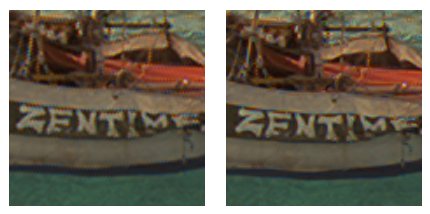
\includegraphics[scale=0.47]{imagenes/Splines/RecortesSplines/pesos1y0/barco2.png}\\
	    PSNR: 27.6018 \ \ \ \ \ \ \ \ \ \ \ \ \ PSNR: 27.5186
	\end{center}
	\begin{center}
	    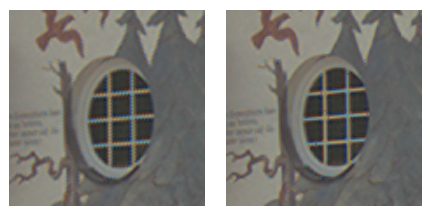
\includegraphics[scale=0.47]{imagenes/Splines/RecortesSplines/pesos1y0/ventana.png}\\
	    PSNR: 26.154 \ \ \ \ \ \ \ \ \ \ \ \ \ PSNR: 25.9947
	\end{center}
	\caption{Combinación de datos mediante promedio (izquierda), y mediante el presente método (derecha)}
	\label{splines3}
\end{figure}

En estas imágenes se evidencia la mejora que brinda el método de las derivadas sobre los bordes de las imágenes. En el primer caso, el texto aparece mucho más nítido, y el \textit{zipper effect} que se podía percibir en los bordes de la franja marrón del barco es mucho menos visible.\\
\indent La segunda imagen, por su parte, también muestra notables mejoras en la ventana: combinando los datos mediante el promedio, podía observarse claramente \textit{zipper effect} y \textit{jaggies} en los bordes internos de la misma; pero al procesar la imagen con el algoritmo que hace uso de las derivadas, las líneas ahora aparecen mucho más suaves y definidas. \\
De todas formas, sigue siendo visible el artifact de Moiré, y pueden verse algunos de los píxeles anormalmente fuertes de los que hablamos antes. \\

\begin{figure}[h!]
	\begin{center}
	    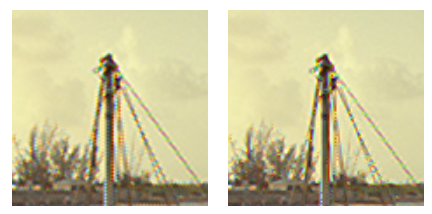
\includegraphics[scale=0.47]{imagenes/Splines/RecortesSplines/pesos1y0/barco1.png}\\
	\end{center}
	\begin{center}
	    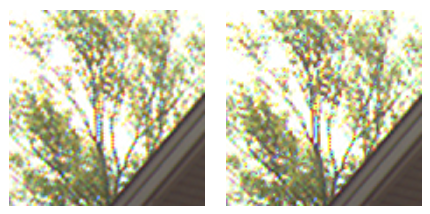
\includegraphics[scale=0.47]{imagenes/Splines/RecortesSplines/pesos1y0/arbol.png}\\
	\end{center}
	\caption{Combinación de datos mediante promedio (izquierda), y mediante el presente método (derecha)}
	\label{splines3}
\end{figure}
\pagebreak
En estas otras dos imágenes pretendemos dejar en evidencia el problema de los píxeles con colores incorrectos. Como puede verse en ambas, las lineas en el caso del segundo método parecen más definidas y con una alta reducción del \textit{zipper effect} y \textit{jaggies}. Sin embargo, puede observarse la presencia de píxeles, sobre todo verdes y rojos, prácticamente saturados, sobre los bordes más finos. \\

Intentando encontrar explicaciones para este fenómeno, concluímos que podía deberse a que estábamos dejando de lado información valiosa a la hora de componer la imagen: sólo usábamos una dirección.\\
\indent Por esta razón, decidimos no arrojar una de las direcciones, sino buscar alguna manera de utilizar ambas para obtener mejoras en la composición.\\
El siguiente método surgió entonces como un intento de mejorar el anterior algoritmo.\\

El mismo consiste en, para cada pixel que no sea verde, calcular los valores resultantes de ambas interpolaciones para el canal verde: tanto la de la fila, como la de la columna, y luego multiplicar a cada uno por algún factor relacionado con las derivadas direccionales de ese mismo canal, en el pixel a estimar.\\

Luego de un análisis sobre qué factor era más conveniente usar, llegamos a la conclusión de que uno inversamente proporcional al valor que tenga cada derivada sería una buena idea. Por lo tanto, definimos:

\[\sigma_G = \partial_xG + \partial_yG \]
\smallskip
\[\alpha_G =
\begin{cases}
0.5 & \sigma_G = 0 \\
  &  \\
1-\frac{\partial_xG}{\sigma_G} & \sigma_G \neq 0
\end{cases}
\]
\medskip
\[\beta_G =
\begin{cases}
0.5 & \sigma_G = 0 \\
  &  \\
1-\frac{\partial_yG}{\sigma_G} & \sigma_G \neq 0
\end{cases}
\]
\pagebreak

En términos implementativos, el algoritmo que resuelve este problema es el siguiente:

\begin{algorithm}[h!]
\NoCaptionOfAlgo
\caption{Algoritmo spline_der (proporcional)}
\For{cada fila de la imagen}{
\eIf{la fila es par}{
\begin{itemize}
\item Generar el spline de toda la fila para el canal azul e interpolar para los píxeles verdes
\item Generar el spline de toda la fila para el canal verde e interpolar para los píxeles azules
\item Multiplicar al resultado de la interpolación anterior por $\alpha$
\end{itemize}
}{
\begin{itemize}
\item Generar el spline de toda la fila para el canal rojo e interpolar para los píxeles verdes
\item Generar el spline de toda la fila para el canal verde e interpolar para los píxeles rojos
\item Multiplicar al resultado de la interpolación anterior por $\alpha$
\end{itemize}
}
}
\bigskip
\For{cada columna de la imagen}{
\eIf{la columna es par}{
\begin{itemize}
\item Generar el spline de toda la columna para el canal rojo e interpolar para los píxeles azules
\item Generar el spline de toda la columna para el canal azul e interpolar para los píxeles verdes
\item Generar el spline de toda la columna para el canal verde e interpolar para los píxeles azules
\item Multiplicar al resultado de la interpolación anterior por $\beta$
\item Sumarlo al valor previo del pixel en el canal verde
\end{itemize}
}{
\begin{itemize}
\item Generar el spline de toda la columna para el canal azul e interpolar para los píxeles rojos
\item Generar el spline de toda la columna para el canal rojo e interpolar para los píxeles verdes
\item Generar el spline de toda la columna para el canal verde e interpolar para los píxeles rojos
\item Multiplicar al resultado de la interpolación anterior por $\beta$
\item Sumarlo al valor previo del pixel en el canal verde
\end{itemize}
}
}
\end{algorithm}

Las imágenes resultantes luego de ser procesadas con el presente algoritmo no produjeron los resultados esperados: las mejoras fueron extremadamente sutiles, al borde de ser indetectables a simple vista, y arrojando resultados de PSNR y SSIM prácticamente idénticos. \\

\textcolor{red}{IMAGENES\\}

Aún más, este algoritmo es considerablemente más lento que el anterior. Teniendo en cuenta el contexto de aplicación, esto no es para nada aceptable: idealmente, un algoritmo de demosaicing debería ser lo suficienteme rápido -o al menos producir imágenes de calidad realmente superior- para justificar el tiempo de cómputo extra requerido.\\

\textcolor{red}{GRAFICO TIEMPO\\}

En conclusión, decidimos descartar este algoritmo: las mejoras eran demasiado sutiles y el tiempo inaceptablemente mayor como para preferirlo.\\

Ya habiendo probado distintas formas de mejorar el algoritmo original (interpolación de una fila y columnas completas, combinando los resultados mediante promedio) y sin obtener resultados considerablemente mejores, decidimos cambiar, no sólo la forma de combinar los resultados, sino también la manera de obtenerlos: nos propusimos dejar de interpolar una fila y columnas completas, y optar por tomar ``rangos'' alrededor de cada pixel sobre los cuales hacer la interpolación. \\

Nuestra hipótesis al plantear esto fue la siguiente: el color de un píxel está definido por un entorno del mismo, es decir, habrá todo un entorno del pixel en donde los colores serán similares (excepto en los bordes). Tiene más sentido estimar el color de un píxel sólo tomando los valores que nos brindan información ``cierta'', y no estimar mediante un polinomio que tiene en cuenta la variación del color a lo largo y ancho de toda la imagen, que puede contener muchos bordes y cambios cromáticos. \\

Para este método seguiremos utilizando la información que nos brindan las derivadas direccionales, más especificamente, utilizar sólo la interpolación de una fila o una columna (en lugar de la técnica proporcional de los pesos), dado que la experimentación antes realizada demostró que el \textit{trade-off} calidad-tiempo beneficia al primero. \\

Además, dado que este método realiza interpolaciones en rangos mucho más chicos (y, por ende, genera Splines mucho más pequeños), esto nos permitió repensar la manera en la que se recorre la imagen, para así intentar realizar una interpolación de mejor calidad para todos los canales: notar que en los métodos explicados hasta el momento, los canales rojo y azul de los píxeles originalmente verdes sólo eran interpolados con la información de las filas (para el canal rojo) o las columnas (para el canal azul), es decir, sólo se interpolaba en una dirección para los colores distintos al verde. Esto se debe a que hubiera sido muy costoso volver a recorrer la imagen, interpolando nuevamente filas y columnas enteras, para interpolar estos canales en las direcciones faltantes.\\

Aún más, dado que ahora le daremos peso a las direcciones de los tres canales por igual, se aplicará el mismo concepto del gradiente para los canales faltantes, notando \(\partial_xB\) y \(\partial_yB\) a las derivadas horizontal y vertical para el canal azul, y \(\partial_xR\) y \(\partial_yR\) a las derivadas horizontal y vertical para el canal rojo.\\

El algoritmo que implementa esta idea se presenta a continuación:
\pagebreak

\begin{algorithm}[h!]
\NoCaptionOfAlgo
\caption{Algoritmo spline_rango}
\For{cada fila de la imagen}{
\If{el pixel actual es azul o rojo}{
Generar un spline de rango $r$ para el canal verde de acuerdo a \(\partial_xG\) y \(\partial_yG\) e interpolar
}
\ElseIf{el pixel actual es verde}{
\eIf{es una fila de verdes y rojos}{
Generar un spline horizontal de rango $r$ para el canal rojo e interpolar\\

Generar un spline vertical de rango $r$ para el canal azul e interpolar
}{
Generar un spline horizontal de rango $r$ para el canal azul e interpolar\\

Generar un spline vertical de rango $r$ para el canal rojo e interpolar
}
}
}
\bigskip
\For{cada fila de la imagen}{
\If{el pixel actual es azul}{
Generar un spline de rango $r$ para el canal rojo de acuerdo a \(\partial_xR\) y \(\partial_yR\) e interpolar
}
\ElseIf{el pixel actual es rojo}{
Generar un spline de rango $r$ para el canal azul de acuerdo a \(\partial_xB\) y \(\partial_yB\) e interpolar}
}
\bigskip
\For{cada fila de la imagen}{
\If{es una fila de verdes y azules, y el pixel actual es verde}{
\If{\(\partial_yR > \partial_xR\)}{
Generar un spline horizontal de rango $r$ para el canal rojo e interpolar
}
\If{\(\partial_xB > \partial_yB\)}{
Generar un spline vertical de rango $r$ para el canal azul e interpolar
}
}
\ElseIf{es una fila de verdes y rojos, y el pixel actual es verde}{
\If{\(\partial_yB > \partial_xB\)}{
Generar un spline horizontal de rango $r$ para el canal azul e interpolar
}
\If{\(\partial_xR > \partial_yR\)}{
Generar un spline vertical de rango $r$ para el canal rojo e interpolar
}
}
}
\end{algorithm}

Donde ``generar un spline de rango $r$ para el canal $C$ de acuerdo a \(\partial_xC\) y \(\partial_yC\) e interpolar'' significa ``calcular la dirección cuya derivada es mayor y generar el spline correspondiente para usar en la interpolación'', como en los métodos anteriores.

\begin{itemize}
\item La primera iteración sobre la imagen se encarga de completar el canal verde para los píxeles distintos del verde, y, para los verdes, completar los canales rojo y azul, sólo en la dirección que tenga información acerca de ese canal (dependerá de la fila en la que se encuentre el pixel verde en cuestión).
\item La segunda iteración se encargará de completar el canal rojo para los píxeles originalmente azules, y el canal azul para los píxeles originalmente rojos. Notar que podemos utilizar las derivadas direccionales también para estos colores porque en el ciclo anterior nos encargamos de que haya información acerca del rojo y el azul en todos los píxeles verdes.
\item Por último, el tercer ciclo se encarga de mejorar la interpolación de los canales rojo y azul para los píxeles verdes. En principio, a los píxeles verdes se les había asignado información del rojo y el azul en una sola dirección, pero ahora, aprovechando que tenemos información del rojo y el azul en todos los píxeles, podemos utilizar el criterio del gradiente para mejorar la estimación.
\end{itemize}


\newpage
\subsection{Algoritmo de Malvar, He y Cutler}

Luego de la lectura y estudio de la publicaci\'on \textit{HIGH-QUALITY LINEAR INTERPOLATION
FOR DEMOSAICING OF BAYER-PATTERNED COLOR IMAGES} \textbf{[2]}, nos decidimos por experimentar con el algoritmo planteado y as\'i observar las mejoras planteadas en este trabajo.\\

Malvar, He y Cutler presentan una cr\'itica a los m\'etodos que no utilizan los tres canales RGB en su conjunto, como por ej. la \emph{interpolaci\'on Bilineal} a la cual le adjudica la generaci\'on de significantes \textit{artifacts}. Y presentan un m\'etodo de Demosaicing en el cual el estudio de cada canal no se hace de manera independiente a los otros dos, que mejora en aspectos de tiempo de c\'omputo a algoritmos similares.\\

Los tres canales en su conjunto contienen informaci\'on sobre la luminiscencia de la imagen, es por esto que al calcular por ej. el valor verde de un p\'ixel orginalmente rojo, se utiliza la informaci\'on contenida en el rojo para la nueva asignaci\'on. Si el valor del p\'ixel rojo difiere de una cantidad significante con sus estimaciones mediante la interpolaci\'on bilineal con sus vecinos, esto significa que hay un cambio abrupto en la luminiscencia y por esto se debe corregir el valor calculado en el canal verde de este p\'ixel a\~nadi\'endole, en proporci\'on, este cambio de luminiscencia.\\

El m\'etodo se basa en una interpolaci\'on bilineal con una correcci\'on respecto al gradiente usando un par\'ametro deseable para controlar cuanta correcci\'on es aplicada.\\

El algoritmo consiste en utilizar una ventana de 5x5, es decir para estimar el valor de un p\'ixel se utilizan los p\'ixeles cercanos dentro del cuadrante con ancho de tama\~no 5 p\'ixeles. Siendo el que est\'a situado en el centro el p\'ixel que va a ser estimado.\\

El algoritmo se comporta de la siguiente manera: situado en un p\'ixel a estimar, se calcula la derivada en su color nativo y luego al calcular los dos canales faltantes se suma esta derivada multiplicada por una constante. De este modo es como se nivela la luminiscencia.\\

Luego de programar el algoritmo y realizar casos de prueba, los resultados arrojados fueron mejores que para los algoritmos anteriores.\\

\textcolor{red}{Poner fotitos y mediciones... no?}\\




\newpage
\section{Resultados y discusi\'on}
\subsection{Exploraci\'on de Artifacts}

\textcolor{blue}{Ver si hay otros artifacts mas para agregar.\\
Ver como arreglar el de Moire y bla...\\
Poner fotitos de ampliaciones donde se vean bien los artifacts.}

EN MHC:\\

Visualmente, podemos definir que las fotos adquirien una mayor definici\'on con contornos menos borrosos e imperfectos. Este algoritmo optimiza la detecci\'on de bordes cuando la diferencia de colores es muy fuerte, por ej. un borde oscuro sobre un fondo claro. Si se comparara con el algoritmo de interpolaci\'on bilineal, en el mismo caso se produc\'ian colores fuertes alrededor de los bordes negros (artifact).

Sim embargo, para los bordes con un menor contraste o bordes m\'as claros, sigue vi\'endose este artifact donde aparecen colores artificiales muy fuertes en la zona de los mismos.

\textcolor{red}{Poner recortes de bordes como estos nombrados arriba}


\newpage
\subsection{An\'alisis cualitativo de los M\'etodos}
Luego de haber generado las im\'agenes con todos los algoritmos que hemos propuesto, nos dispusimos a correr en Matlab$\textregistered$  la diferencia (resta) entre ellas y la imagen original de la cual partimos. Luego de eso, invertimos los colores para poder apreciar mejor d\'onde se notaban las mayores diferencias. A continuaci\'on se incluyen las im\'agenes obtenidas con este proceso, en color blanco y negro con el objetivo de distinguir id\'oneamente las regiones de la imagen donde exista un error contundente.\\


\begin{figure}[h!]
    \caption{}
    \begin{center}
    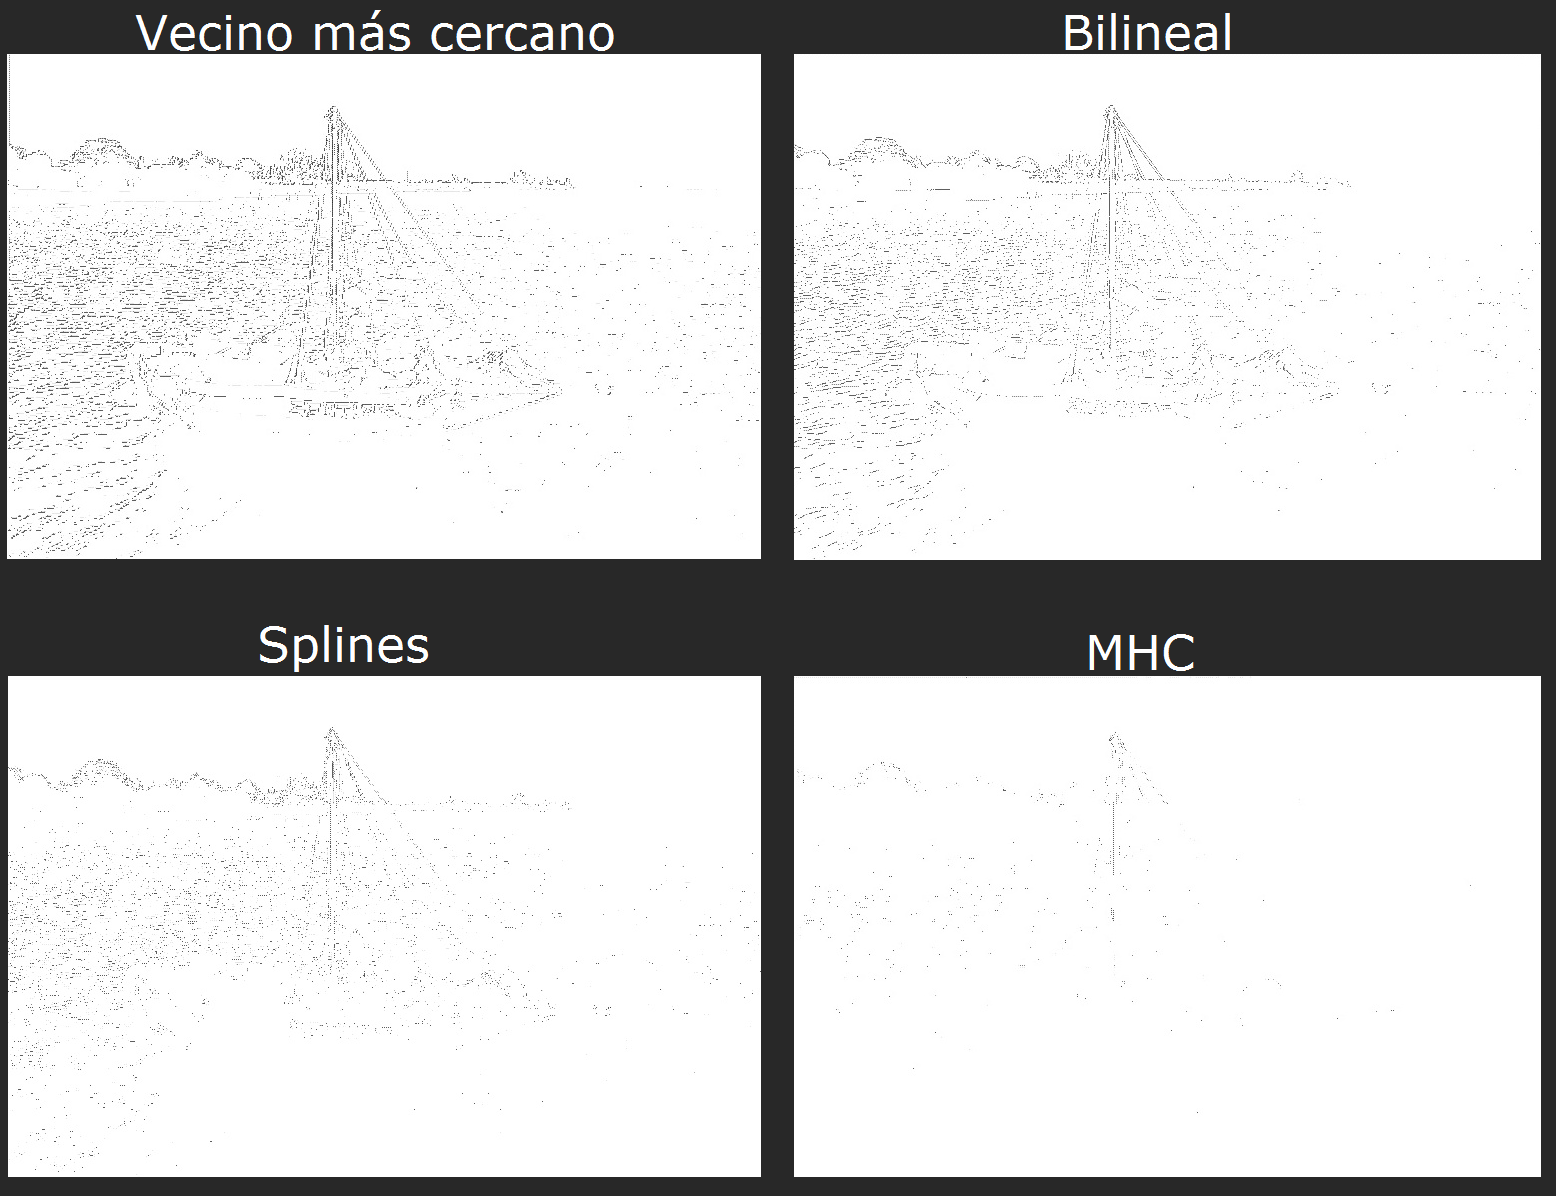
\includegraphics[scale=0.40]{imagenes/comparacion/02/collage}
    \label{imagen2}
  \end{center}
\end{figure}


\newpage

\begin{figure}[h!]
    \caption{Imagen Original}
    \begin{center}
    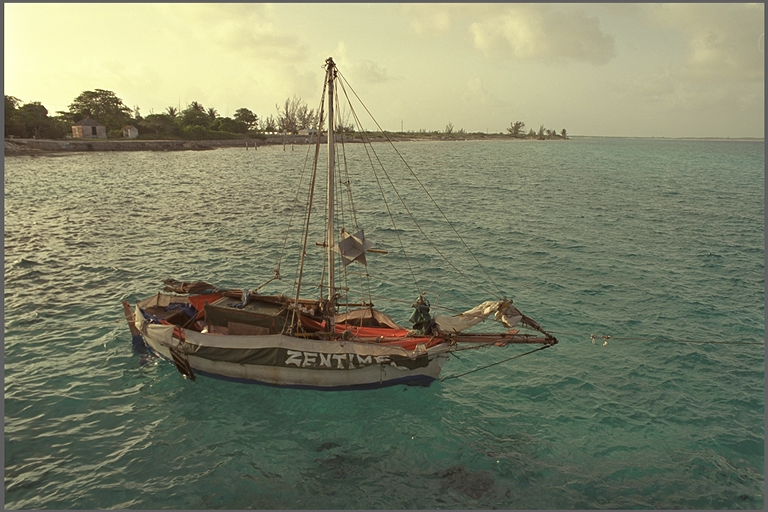
\includegraphics[scale=0.15]{imagenes/comparacion/02/img2}
    \label{imgOri2}
  \end{center}
\end{figure}

En la Figura \ref{imagen2}  se puede observar que, si bien al ejecutar el algoritmo de MHC disminuye abundantemente la diferencia con la imagen original, al tener una superficie en su mayor\'ia de agua se dificulta a niveles algor\'itmicos aproximar el agua de una manera m\'as real ya que esta no es para nada una superficie pareja. Estas diferencias tal vez no sean tan visibles al ojo humano, pero en cuanto a diferencia de color p\'ixel a p\'ixel es notorio.

 Tambi\'en se hace presente el artifact que hay sobre la punta superior del mastil, dado que se puede observar la anomalía en los cuatro algoritmos. En un primer momento, se puede apreciar Zipper y Moir\'e
(en el algoritmo de Vecino M\'as Cercano) y a medida que se van utilizando m\'etodos ``mejores'' este artifact se reduce simplemente a un peque\~no Moir\'e. \\


\begin{figure}[h!]
    \caption{Zoom en imágenes obtenidas mediante los distintos métodos}
    \begin{center}
    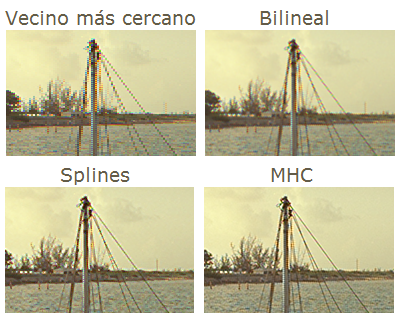
\includegraphics[scale=1.2]{imagenes/comparacion/02/mastil}
    \label{mastil}
  \end{center}
\end{figure}

\newpage

\begin{figure}[h!]
    \caption{Imagen Original}
    \begin{center}
    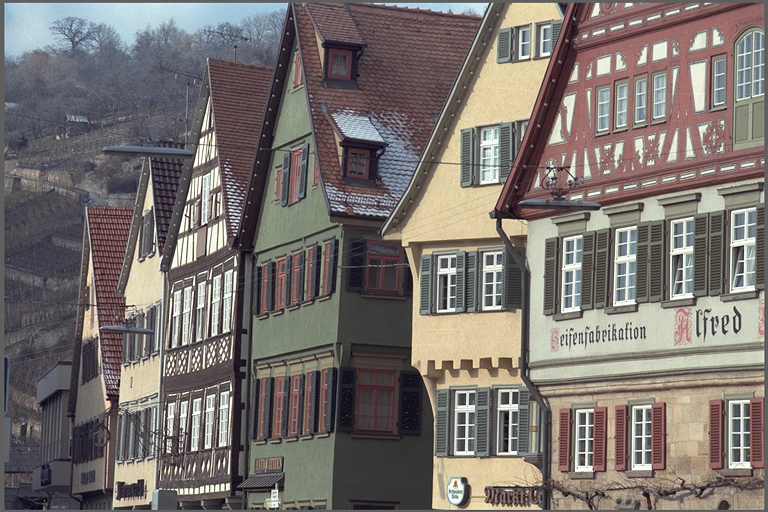
\includegraphics[scale=0.15]{imagenes/comparacion/04/img4}
    \label{imagen4}
  \end{center}
\end{figure}

\begin{figure}[h!]
    \caption{}
    \begin{center}
    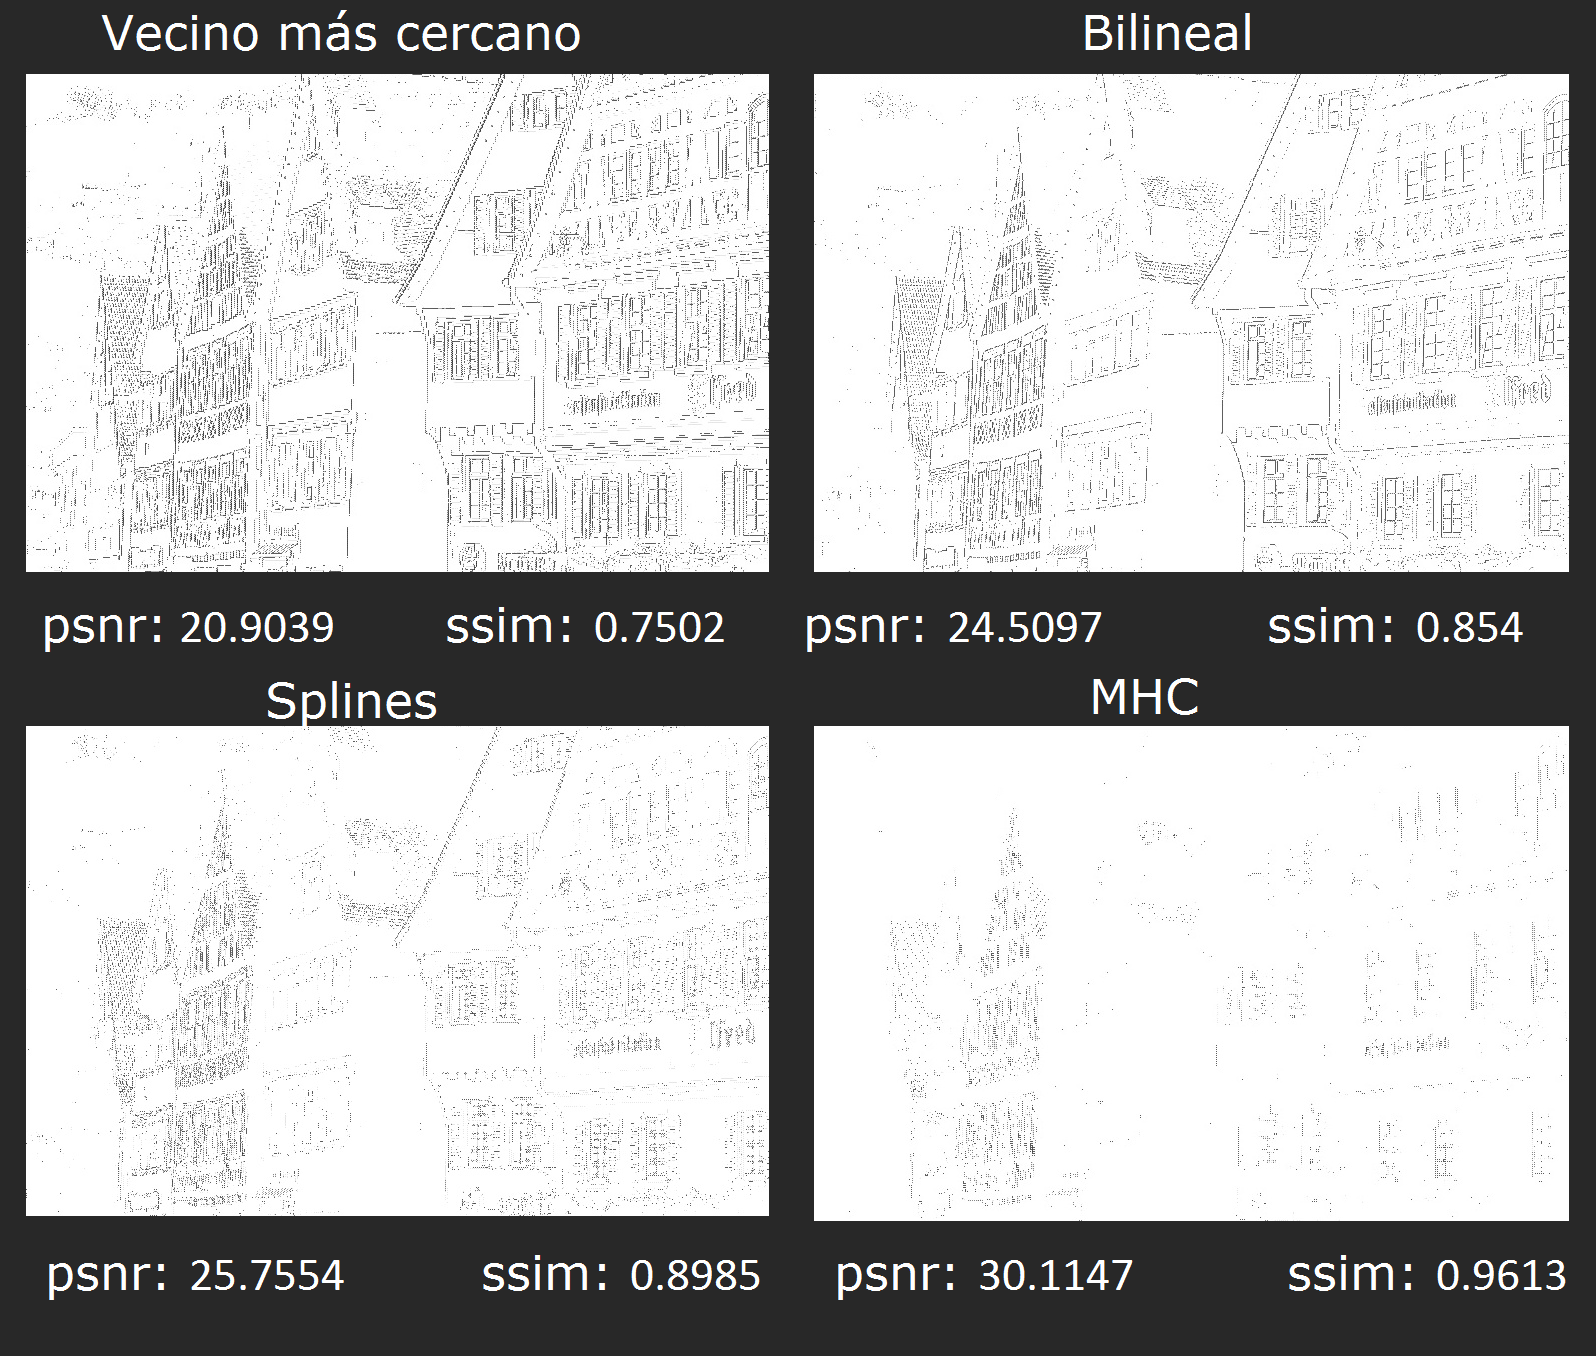
\includegraphics[scale=0.40]{imagenes/comparacion/04/collage}
    \label{imagen4}
  \end{center}
\end{figure}

En la Figura \ref{imagen4} se puede apreciar el inconveniente de aproximar p\'ixeles que son borde cuando estos son dados en abundancia y en l\'ineas recta en su mayor\'ia. Inclusive en el mejor caso de esta imagen, (la imagen creada mediante el Algoritmo de MHC) se puede apreciar una notable diferencia con la original en lo que respecta a los bordes.\\

Si ahondamos en la imagen, notamos que es en las ventanas donde perciste el problema para todos los métodos. Si nos detenemos en la imagen obtenida se puede apreciar un artifact en específico: Moir\'e. \\

\begin{figure}[h!]
    \caption{Zoom en imágenes obtenidas mediante los distintos métodos}
    \begin{center}
    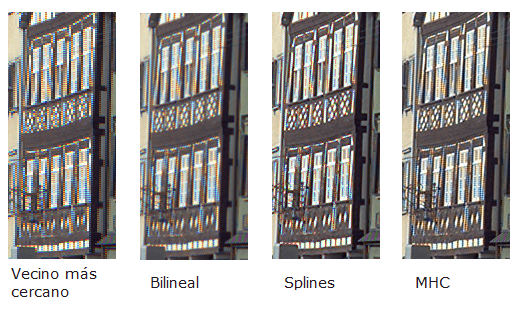
\includegraphics[scale=1]{imagenes/comparacion/04/ventanitas}
    \label{ventanitas}
  \end{center}
\end{figure}

El otro inconveniente presente se ubica en el letrero, el cual gradualmente adquiere mayor definici\'on, pero as\'i mismo persiste marcandose la diferencia con el original. \\

\begin{figure}[h!]
    \caption{Zoom en imágenes obtenidas mediante los distintos métodos}
    \begin{center}
    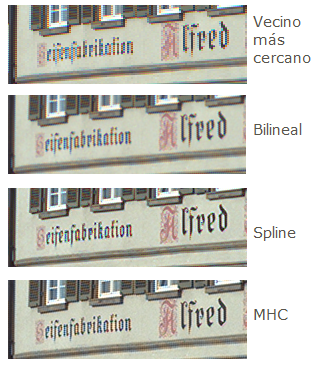
\includegraphics[scale=0.9]{imagenes/comparacion/04/letrero}
    \label{letrero}
  \end{center}
\end{figure}

\newpage

\begin{figure}[h!]
    \caption{Imagen Original}
    \begin{center}
    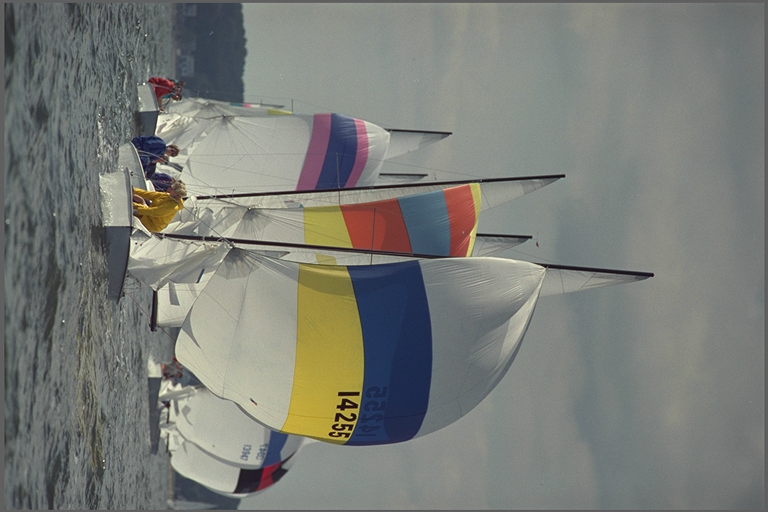
\includegraphics[scale=0.15]{imagenes/comparacion/05/img5}
    \label{imgOri2}
  \end{center}
\end{figure}

\begin{figure}[h!]
    \caption{}
    \begin{center}
    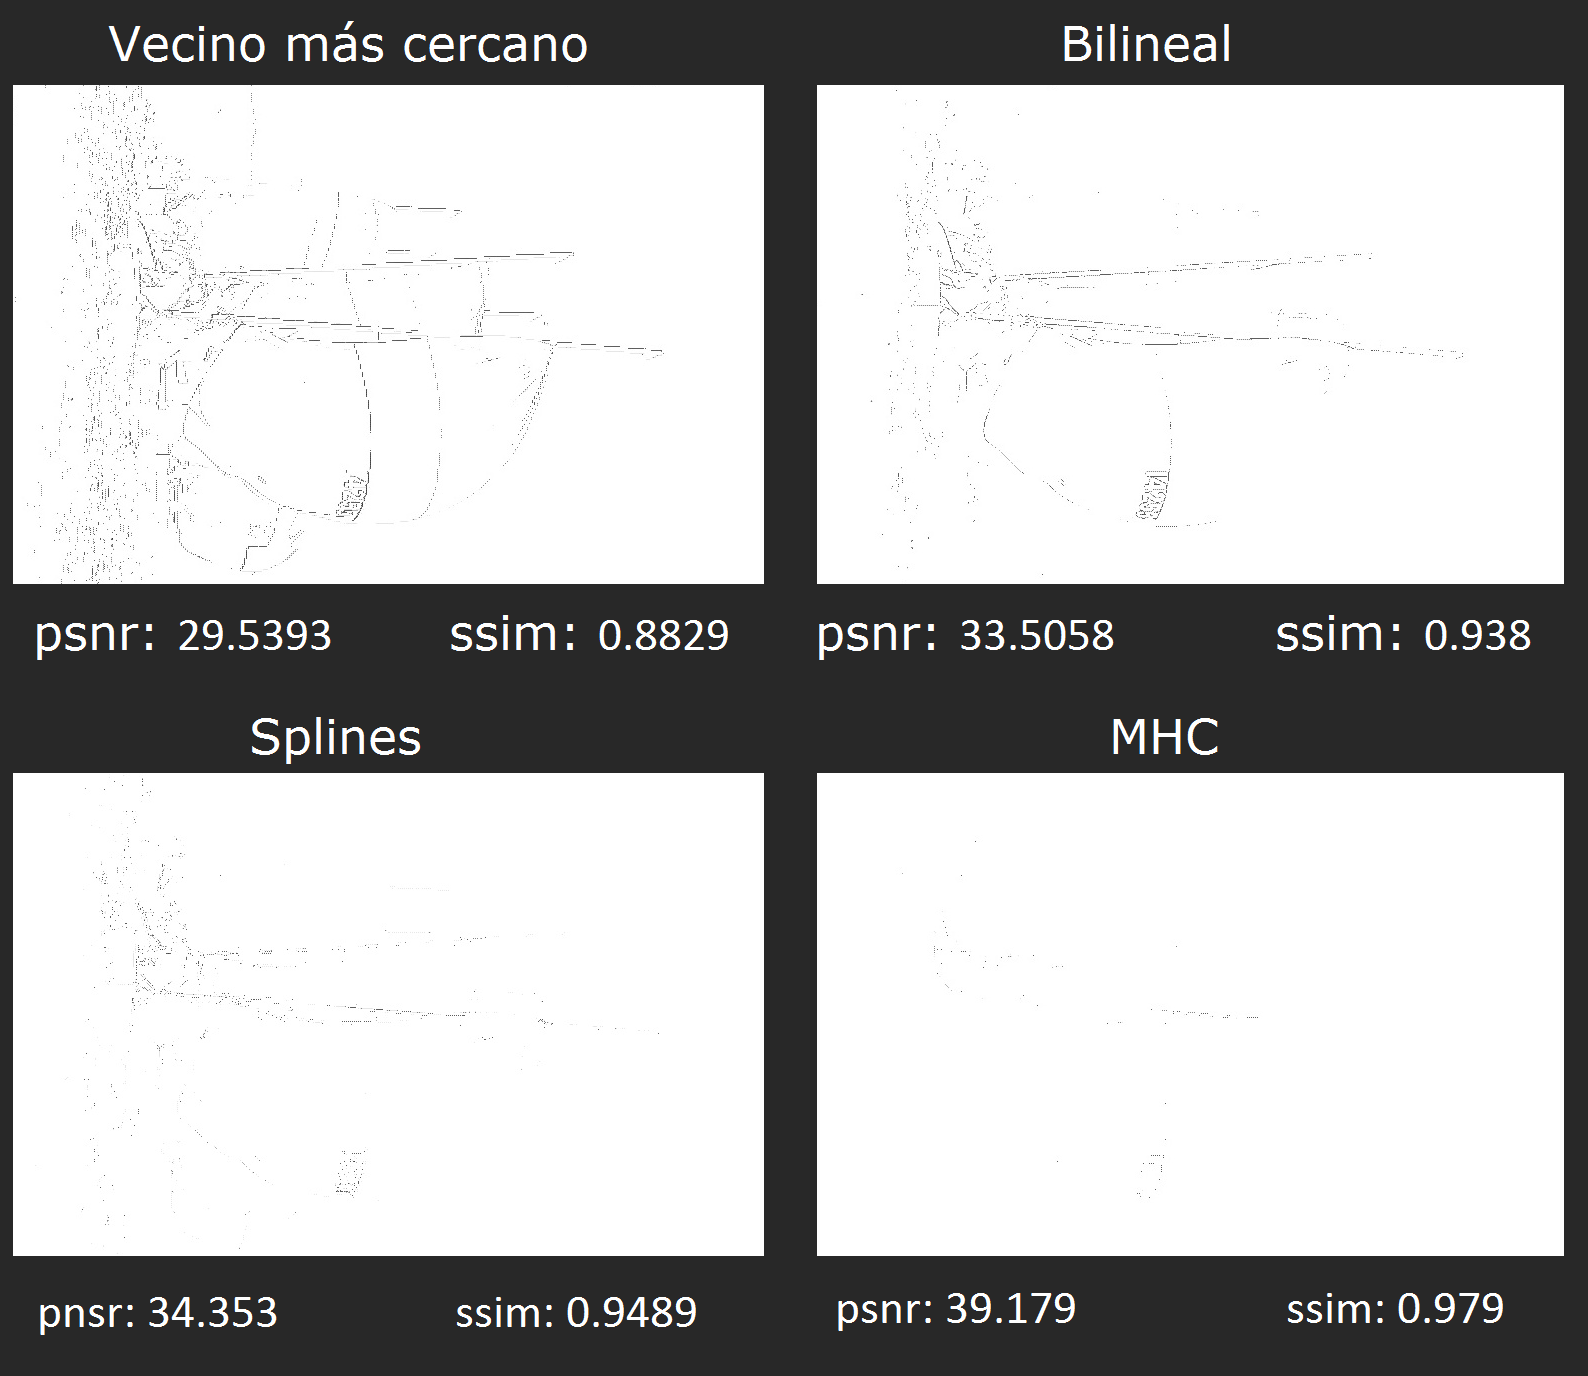
\includegraphics[scale=0.40]{imagenes/comparacion/05/collage}
    \label{imagen5}
  \end{center}
\end{figure}


En cuanto a la Figura \ref{imagen5} se puede notar un comportamiento similar al de la imagen en la Figura \ref{imagen2} dado a la existencia de agua, la cual es una superficie dif\'icil de estimar para los m\'as b\'asicos algoritmos.\\

Lo interesante a destacar de este caso, es el gran avance que se realiza mediante el algoritmo de MHC en contraposici\'on de los otros dos. Se puede apreciar que las diferencias entre la imagen estimada por este algoritmo y la imagen original se convierten en \'infimas.


\newpage

\begin{figure}[h!]
    \caption{Imagen Original}
    \begin{center}
    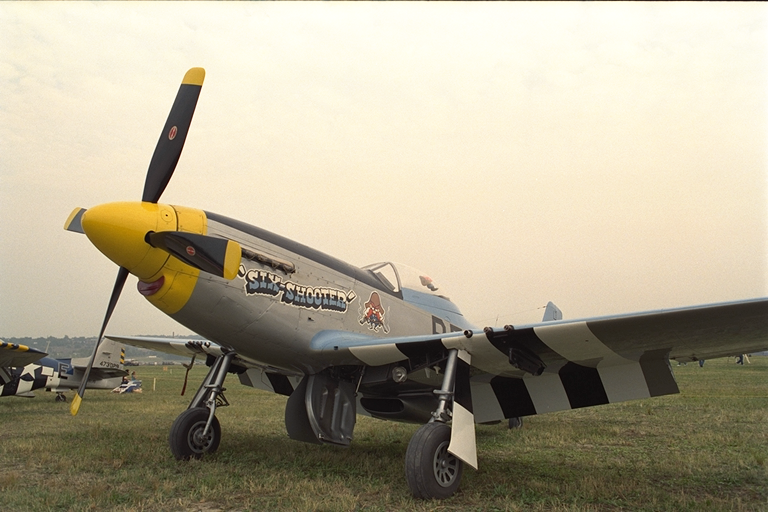
\includegraphics[scale=0.15]{imagenes/comparacion/09/img9}
    \label{imgOri2}
  \end{center}
\end{figure}

\begin{figure}[h!]
    \caption{}
    \begin{center}
    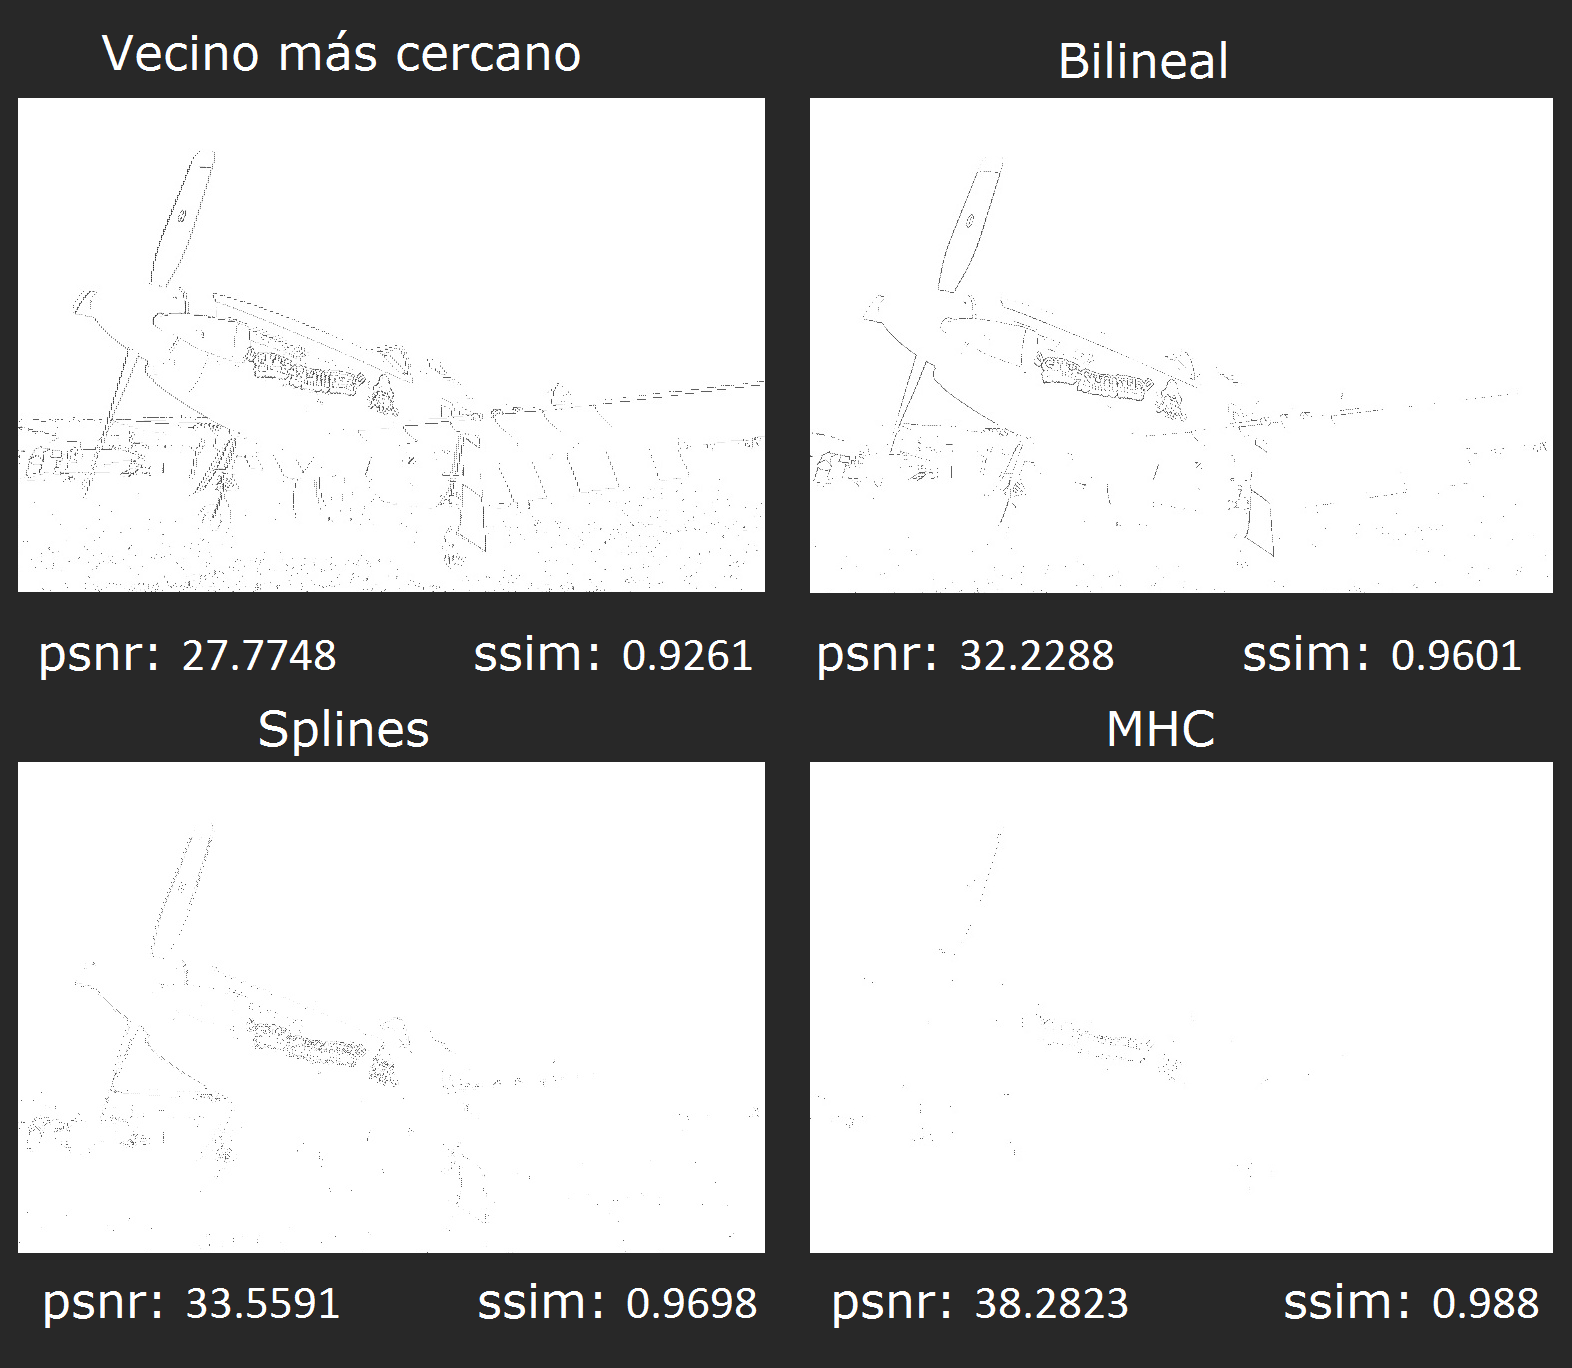
\includegraphics[scale=0.40]{imagenes/comparacion/09/collage}
    \label{imagen9}
  \end{center}
\end{figure}

\newpage

En la Figura \ref{imagen9} se puede ver un comportamiento similar a lo ya estudiado, lo interesante de destacar en cuanto a esta foto es que al poseer un letrero es una imagen menos abstracta que las anteriores y por lo tanto, se adquiere una definici\'on mayor cuando se tiene una diferencia menor con la original y as\'i facilitar la lectura del cartel.



\begin{figure}[h!]
    \caption{Zoom en imágenes obtenidas mediante los distintos métodos}
    \begin{center}
    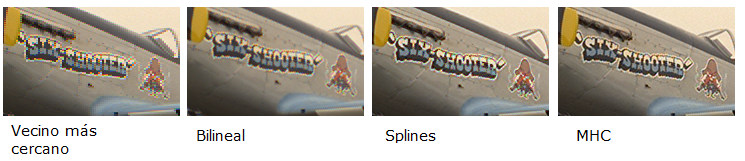
\includegraphics[scale=0.9]{imagenes/comparacion/09/cartel}
    \label{cartel}
  \end{center}
\end{figure}

\newpage

\begin{figure}[h!]
    \caption{Imagen Original}
    \begin{center}
    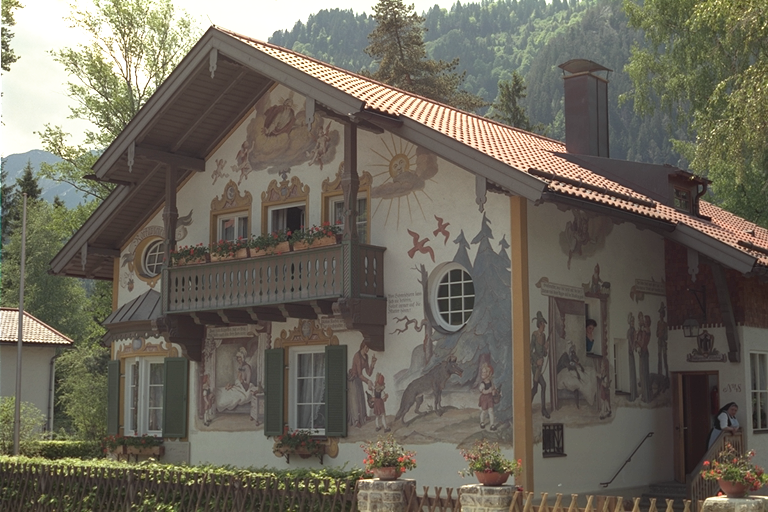
\includegraphics[scale=0.15]{imagenes/comparacion/12/img12}
    \label{imgOri2}
  \end{center}
\end{figure}

\begin{figure}[h!]
    \caption{}
    \begin{center}
    \includegraphics[scale=0.40]{imagenes/comparacion/12/collage}
    \label{imagen12}
  \end{center}
\end{figure}

La Figura \ref{imagen12} es una imagen con muchas l\'ineas y dibujos con contornos. Esto se aprecia en la gran densidad que tiene la imagen que muestra las diferencias entre la imagen original y la imagen obtenida  mediante el algoritmo de Vecino M\'as Cercano. Si observamos las im\'agenes obtenidas mediante la resta con sus respectivas originales se denota una gran diferencia entre el Algoritmo de Vecino M\'as Cercano y el Algoritmo de MHC.\\

\newpage

\begin{figure}[h!]
    \caption{Zoom en imágenes obtenidas mediante los distintos métodos}
    \begin{center}
    \includegraphics[scale=0.9]{imagenes/comparacion/12/techo}
    \label{imagen12}
  \end{center}
\end{figure}


\begin{figure}[h!]
    \caption{Zoom en imágenes obtenidas mediante los distintos métodos}
    \begin{center}
    \includegraphics[scale=1.1]{imagenes/comparacion/12/ventanita}
    \label{imagen12}
  \end{center}
\end{figure}

En la secci\'on de la foto que le corresponde al techo se puede apreciar el artifact de \emph{False Colors}. Ya que aparecen p\'ixeles con tonos y colores que no corresponden a la imagen original. Se puede apreciar como, gradualmente, esta anomal\'ia va desapareciendo otorg\'andole a la imagen mayor nitidez. Por este motivo, se podr\'ia decir tambi\'en que MHC elimina el artifact \emph{mblur}, al menos en este caso.\\

La ventana es un punto de an\'alisis importante ya que las dos primeras estimaciones producen Zipper, mientras que con Splines disminuye hasta la casi inexistencia no llega a estimarse a la perfecci\'on. En el caso de MHC se podr\'ia decir que la ventana se ve con una similitud importante respecto de la imagen original.

\newpage

Nos pareci\'o un caso de inter\'es lo ocurrido en la siguiente imagen:
\begin{figure}[h!]
    \caption{Imagen Original}
    \begin{center}
    \includegraphics[scale=0.15]{imagenes/comparacion/07/img7}
    \label{imgOri2}
  \end{center}
\end{figure}

\begin{figure}[h!]
    \caption{}
    \begin{center}
    \includegraphics[scale=1]{imagenes/comparacion/07/palmeritas}
    \label{palmas}
  \end{center}
\end{figure}

\newpage

En la Figura \ref{palmas} cabe destacar dos aspectos:

\begin{itemize}
\item \textbf{Nitidez de los troncos de las palmeras}: En esta imagen se repite algo que observamos en casos anteriores. El algoritmo de Vecino m\'as cercano produce Zipper notablemente y a medida que se avanza con los algoritmos, este artifact decrementa su existencia. De este modo, lo que sol\'ia ser una l\'inea inexacta y con colores pocos reales termina convirti\'endose en un tronco muy cercano en aspecto al de la imagen original. 
\item \textbf{False colors}: Algo llamativo que acontece con esta foto es la aparici\'on de una espuma turquesa en la orilla. Si bien bajo el algoritmo de Vecino m\'as cercano posee una pronunciaci\'oon mayor ning\'un algoritmo es capaz de eliminarla del todo. Los resultados obtenidos difieren bastante visualmente de la imagen original. Esta aparici\'on de un color que no existe es un caso m\'as del artifact False Colors.
\end{itemize}

\newpage


Como conclusi\'on, podemos inferir que los lugares donde se muestra una variaci\'on son siempre lugares pertencientes a contornos o bordes de objetos en las im\'agenes. En cambio, en p\'ixeles sobre superficies llanas o parejas del mismo cuerpo la diferencia entre la imagen original y nuestra imagen obtenida es casi nula.\\

Y tambi\'en se puede concluir que para todos los casos de test realizados, coincide que el algoritmo \'optimo es el de MHC.\\

\textit{Se adjuntan las im\'agenes en su tama\~no original.}


\newpage
En las siguientes figuras se puede observar como aumentan, acorde al m\'etodo, los valores de psnr y ssim.
\begin{figure}[h!]
    \caption{Evaluaci\'on de psnr para 12 im\'agenes del mismo tama\~no}
    \begin{center}
    \includegraphics[scale=0.75]{imagenes/graficos/psnr}
    \label{psnr}
  \end{center}
\end{figure}

\begin{figure}[h!]
    \caption{Evaluaci\'on de ssim para 12 im\'agenes del mismo tama\~no}
    \begin{center}
    \includegraphics[scale=0.75]{imagenes/graficos/ssim}
    \label{ssim}
  \end{center}
\end{figure}

\newpage
\subsection{An\'alisis de tiempos}
\textcolor{blue}{Aca hay que comparar los tiempos de ejecucion entre todos los algoritmos dispuestos.}

\newpage
\section{Conclusiones y trabajo futuro}

Es importante conocer nuestras limitaciones. Si bien bajo el algoritmo de MHC la existencia de \emph{Artifacts} es casi nula, hay algunos que persisten y la forma de solucionar esto excede a nuestro trabajo. Por este motivo, nos centraremos en el \'optimo m\'etodo para resolver el \emph{Demosaicing} sin esperar que este sea infalible y meramente real.\\

Como primera instancia, el Algoritmo de\textit{ Vecino M\'as Cercano} es capaz de esbozar la estructura de la imagen a grandes rasgos. Sin embargo, los bordes no suelen ser muy precisos y la definici\'on tiende a ser de baja calidad. Sumado a que es el m\'etodo donde encontramos mayor diversidad de Artifacts y mayor ocurrencia bajo una misma imagen. Cabe destacar que los valores de psnr y ssim arrojados en nuestra experimentaci\'on para este m\'etodo fueron siempre los menores.\\

La interpolaci\'on Bilineal tiende a ser una buena soluci\'on respecto de los contornos cuadrados que se generan bajo el m\'etodo de Vecino m\'as cercano, ya que admite un dibujo de contornos m\'as flexible aunque no \'optimo.\\

Los splines bla...\\

Con los resultados arrojados por nuestra experimentaci\'on nos vemos condicionados a determinar que el m\'etodo \'optimo entre los cuatro probados es el del Algoritmo de Malvar, He y Cutler. Este m\'etodo es el que mejores n\'umeros obtuvo de psnr y ssim para todos los casos evaluados. Adem\'as, es el m\'etodo donde encontramos menor diversidad de artifacts y, sobre todo, menor cantidad de artifacts en una misma imagen. \\

\textcolor{red}{Ademas de completar los puntos suspensivos, hay que agregar algo respecto del tiemmpo empleado por cada uno y si vale la pena esperar o no y bla...\\
Tambi\'en poner que los valores de ssim y psnr fueron constantes, es decir siempre en el mismo orden.}\\

No hay que perder de vista que la implementaci\'on deber\'a ser ejecutada en tiempo real, lo cual implica que si un algoritmo es muy bueno para la estimaci\'on de la imagen pero tarda un tiempo considerablemente alto no es realmente el \'optimo.




\section{Ap\'endices}
\subsection{Ap\'endice A: Enunciado} 

%ACORDARSE DE DESCOMENTARLO%%%%%%%%%%%%%%%%%%%%%%%%%%%%%%%%%%%%%%%%%%%%%%%%%%%%%%%%%%%%%

%\includepdf[pages={-}]{Enunciado.pdf}

\subsection{Ap\'endice B:}
\newpage
\section{Referencias}
 
\textbf{[1]} Ron Kimmel. Demosaicing: image reconstruction from color ccd samples. \textit{IMAGE PROCESSING, IEEE TRANSACTIONS ON}, 1999. \\
\\

\textbf{[2]} Henrique S. Malvar, Li wei He, and Ross Cutler. High-quality linear interpolation for
demosaicing of bayer-patterned color images. In \textit{Proceedings of the IEEE International
Conference on Speech, Acoustics, and Signal Processing}, 2004.\\
\\

\textbf{[3]} R. Burden y J.D.Faires, \textit{An\'alisis num\'erico}, International Thomson Editors, 1998

\end{document}

%%%%%%%%%%%%%%%%%%%%%%%%%%%%%%%%%%%%%%%%%%%%%%%%%%%%%%%%%%%%%%%%%%%%%%%%%
\begin{figure}
  \begin{center}
	\includegraphics[scale=0.66]{imagenes/logouba.jpg}
	\caption{Descripcion de la figura}
	\label{nombreparareferenciar}
  \end{center}
\end{figure}


\paragraph{\textbf{Titulo del parrafo} } Bla bla bla bla.
Esto se muestra en la figura~\ref{nombreparareferenciar}.



\begin{codesnippet}
\begin{verbatim}

struct Pepe {

    ...

};

\end{verbatim}
\end{codesnippet}
